\documentclass[12pt,a4paper]{report}
\usepackage[utf8]{inputenc}
\usepackage[T1]{fontenc}
\usepackage{boldline,multirow,tabularx,colortbl,diagbox,makecell,fancybox}
\usepackage{amsfonts,amssymb,amsmath,mathrsfs,array,stmaryrd}
\usepackage{pgf,tikz,xcolor}
\usetikzlibrary{calc,positioning,shapes.geometric,shapes.symbols,shapes.misc, fit, shapes, arrows, arrows.meta,fadings,through}
\usepackage[top=2.5cm, bottom=2.5cm, left=2.5cm, right=2.5cm]{geometry}
\usepackage{fancyhdr}
\usepackage{hyperref}
\usepackage[french]{babel}
\usepackage{graphicx}
\usepackage{booktabs}
\usepackage{float}
\usepackage{subfigure}
\usepackage{wrapfig}
\usepackage{biblatex}
\usepackage{booktabs}
\usepackage{array}
\usepackage{algorithme}
\usepackage{csquotes}
\usepackage[inkscapelatex=false]{svg}
\usepackage{pdflscape}
\usepackage{pdfpages}
\usepackage[
    left = \flqq{},% 
    right = \frqq{},% 
    leftsub = \flq{},% 
    rightsub = \frq{} %
]{dirtytalk}

\geometry{margin=2.5cm}

\begin{document}

\pagenumbering{gobble}
\thispagestyle{empty}
\noindent\begin{tikzpicture}[remember picture, overlay, shift={(current page.south west)}]
    \node[anchor=north west] at (2,27.7) {
\includegraphics[height=1.225cm, keepaspectratio]{INSALogo.pdf}};
    \node[anchor=north west] at (2,26.25) {Département ITI};
    \node[above = 90pt of current page.center] (ptitle) {\parbox{\textwidth}{\centering\LARGE{\textbf{Rapport de projet}\\
    \text{Smart Robot}
    }}};
    \node[above = 12.5pt of ptitle.north] {\rule{4cm}{0.25mm}};
    \node[below = 12.5pt of ptitle.south] {\rule{4cm}{0.25mm}};
    
    \node[above = 230pt of current page.center] (rapport) {\Large{\textsc{Projet intégratif : Smart Robot}}};
    \node[below = 65pt of current page.center] (pstudents) {\centering\begin{tabular}{ll}
        Célia & ANTUNES \\
        Edouard & DOUBET \\
        Adam & EL MARZOUKI \\
        Bréhan & ERAUD-ROBERT \\
        Hadi & ASSI \\
        Romain & LEPREVOST \\
    \end{tabular}};
    \node[above = 5pt of pstudents] (pstudentstitle) {\textbf{Étudiants}};
    
    \node[below = 150pt of pstudents] (pdate) {\today};
\end{tikzpicture}

\newpage
\tableofcontents
\newpage
\pagenumbering{arabic}

% -------------------------------
% INTRODUCTION
% -------------------------------
\chapter*{Introduction}
\addcontentsline{toc}{chapter}{Introduction}

Dans le cadre de ce projet intégratif, nous étions chargés de concevoir un robot capable de répondre à une problématique imposée. Ce projet avait pour objectif de mettre en \oe uvre les différentes compétences acquises lors du cours d'Algorithmique ainsi que celui d'Électronique pour les systèmes embarqués. La gestion de projet était également importante pour assurer le suivi et la coordination des différentes étapes du projet.\\


\noindent Ce projet se divise en deux parties complémentaires. La première partie est une partie algorithmique, qui consiste en l'analyse de la description de la ville. Afin de déterminer le parcours le plus optimal, et préparer une liste d'instructions pour le robot. La deuxième partie est une partie robotique, qui consiste à concevoir le robot, et faire un programme capable de le piloter, et d'exécuter les différentes instructions générées lors de la première partie.\\

\noindent Le cahier des charges pour le projet sera le suivant :
\begin{itemize}
    \item Le robot doit être capable de suivre des lignes noires et de corriger sa trajectoire en cas de déviations.
    \item Le robot doit être capable de franchir un certain nombre de points de passage imposés.
    \item Le robot doit être capable de revenir à son point de départ.
    \item L'algorithme doit être capable de trouver le parcours le plus court possible.
\end{itemize}

\vspace{1cm}

\noindent Le rapport sera donc structuré de la manière suivante. Dans une première partie, nous présenterons, de manière plus détaillée les contraintes techniques du sujet, l'organisation du projet et les différentes étapes de conception. Dans une seconde partie, nous présenterons la conception électronique du robot, incluant le schéma électrique, les choix techniques et le bilan de puissance du robot. Ensuite, nous aborderons dans la troisième partie, les choix de conception et d'implémentation de notre robot. Celui-ci suivra le cycle en V, et abordera les algorithmes clés. Dans un dernier temps, nous ferons un bilan de la démonstration, avec un commentaire sur les performances du robot, et d'éventuels problèmes rencontrés. Enfin, nous ferons une synthèse du projet, en abordant les différents problèmes rencontrés et les solutions proposées à une échelle plus globale.\\


% -------------------------------
% CHAPITRE 1 — Présentation du sujet
% -------------------------------
\chapter{Présentation du sujet}

\section{Description générale du problème}
Dans cette partie, nous allons passer en revue les différentes contraintes imposées, et l'organisation générale de notre groupe dans le cadre du projet. Le but n'est pas d'aborder en détail ce que nous avons réalisé, mais plutôt de passer en revue le déroulement général du projet.


\section{Format du fichier de description de la ville}
L'entrée pour notre programme sera un fichier texte décomposé comme suit :
\begin{itemize}
    \item Première ligne : largeur $l$ (nombre de cases par côté).
    \item Deuxième ligne : case de départ + orientation (par exemple \texttt{6S}).
    \item Lignes suivantes : passages entre cases (\texttt{1-2}, \texttt{1-6}, etc.).
    \item Dernières lignes : numéros des cases contenant les points de passage.
    \item Fin du fichier : un point \texttt{.}.
\end{itemize}

\hspace{1cm}

\noindent Ce fichier sera lu par notre programme pour comprendre la ville et les points de passage, une fois le programme terminé, il renverra une liste d'instructions pour le robot. Regardons donc un peu plus en détail quels sont les ordres que le robot peut recevoir.

\section{Différents ordres pour le robot}
\begin{itemize}
    \item \texttt{AV} : avancer jusqu'au prochain croisement ;
    \item \texttt{TG} : tourner à gauche (sans avancer) ;
    \item \texttt{TD} : tourner à droite (sans avancer).
\end{itemize}

\hspace{1cm}

\noindent Ces ordres seront lus par notre programme et exécutés par le robot pour réaliser le parcours complet. Le programme de création des instructions lit un fichier, spécifié en paramètre de la commande, afin d'obtenir les informations de la ville. Son exécution produit une sortie dans la sortie standard, que nous récupérons dans l'entrée standard du programme chargé de déplacer le robot. L'exécution des programmes ressemble donc à \texttt{./algo/bin/laby ville.txt | ./elec/bin/robot}.

% -------------------------------
% CHAPITRE 2 — Partie électronique
% -------------------------------
\chapter{Partie électronique}

\section{Schéma électrique}
\begin{figure}[H]
    \centering
    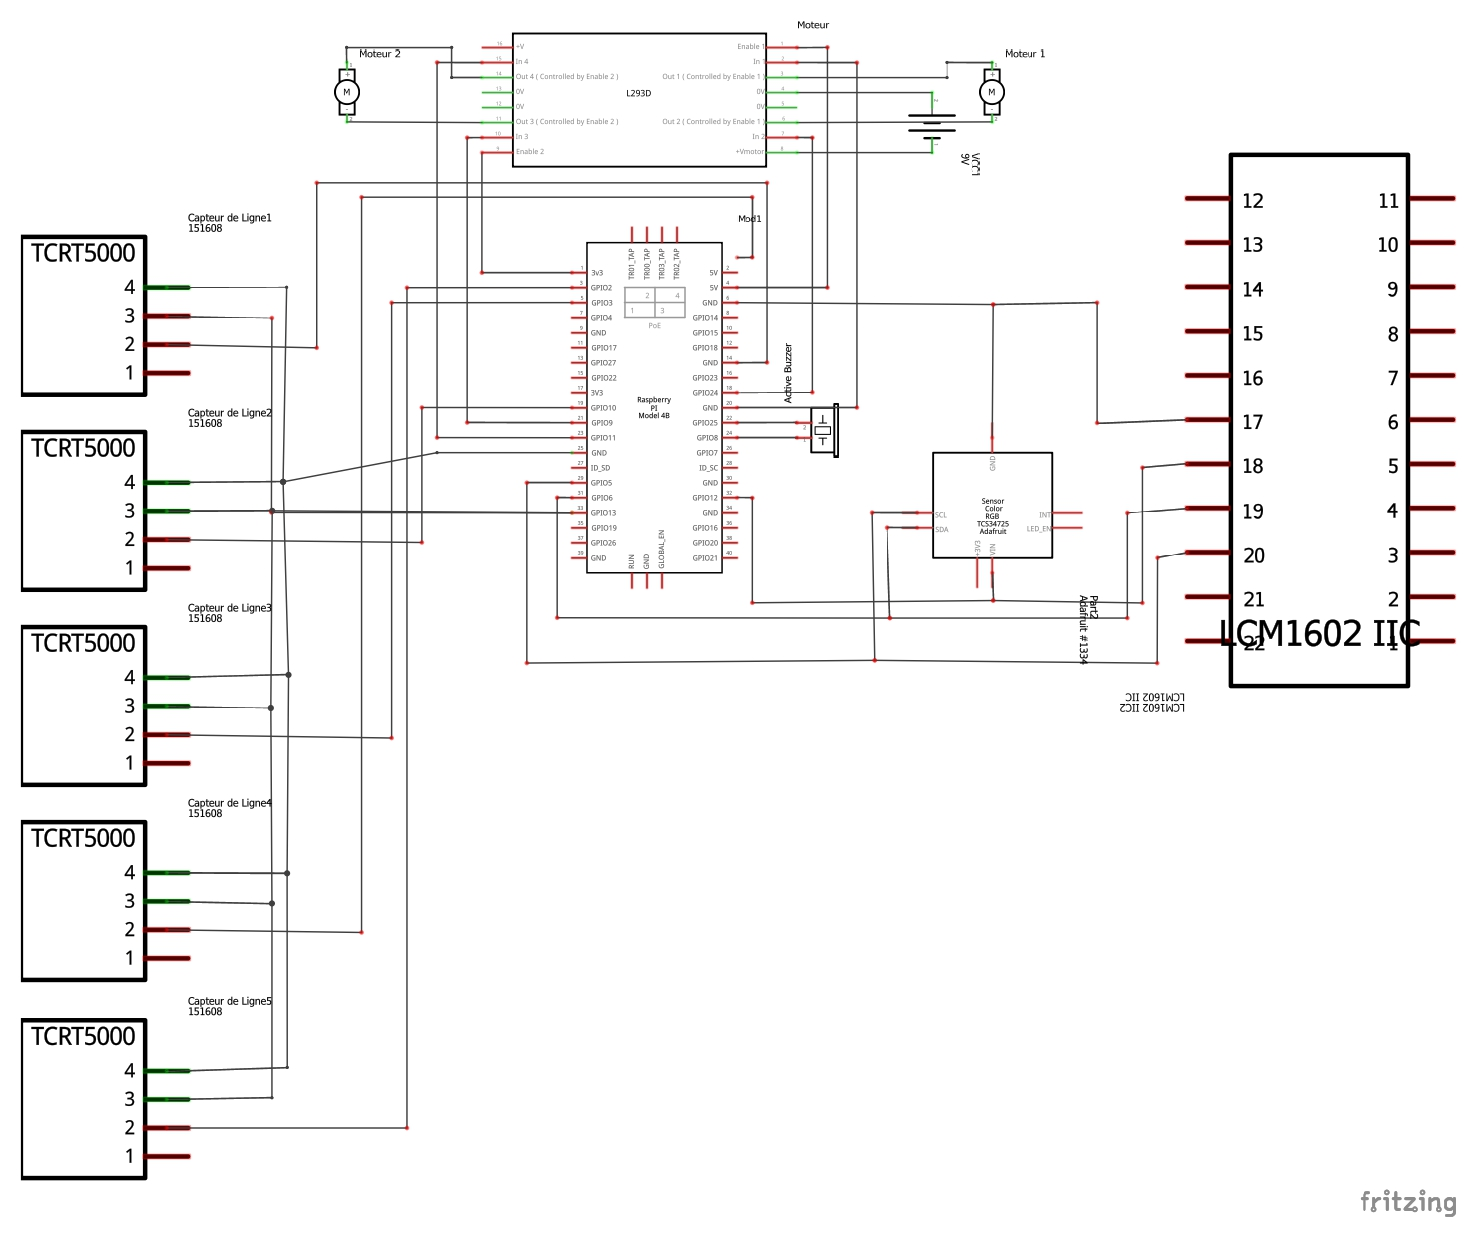
\includegraphics[width=0.9\textwidth]{parties/schema_electrique.jpg}
    \caption{Schéma électrique complet du robot.}
\end{figure}
% Si vous voulez, vous pouvez rediriger ici vers le doc fritzing au lieu d'un ong
Le module I2C, sur la boîte est normalement branché à l'écran LCD, mais il n'est pas branché par lisibilité du schéma, et que notre module était déjà branché de notre côté.
%hadi---

\section{Architecture matérielle du robot}

\subsection{Raspberry Pi : cœur du système}

\subsubsection{Rôle}
Le Raspberry Pi constitue le cerveau du robot. Il assure les fonctions suivantes :
\begin{itemize}
    \item lecture des données provenant des capteurs,
    \item traitement des informations,
    \item commande des moteurs,
    \item communication avec l’écran LCD et le capteur de couleur.
\end{itemize}

\subsubsection{Connexions principales}
\begin{itemize}
    \item GPIO $\rightarrow$ capteurs de ligne TCRT5000,
    \item GPIO $\rightarrow$ driver de moteurs L293D,
    \item GPIO I2C (SDA, SCL) $\rightarrow$ écran LCD et capteur de couleur,
    \item GPIO $\rightarrow$ buzzer,
    \item Alimentation 5V et GND $\rightarrow$ ensemble des modules.
\end{itemize}

%-------------------------------------------------

\subsection{Capteurs de ligne TCRT5000 (x5)}

\subsubsection{Rôle}
Les capteurs TCRT5000 sont des capteurs infrarouges utilisés pour :
\begin{itemize}
    \item détecter une ligne noire sur un fond clair (suivi de ligne),
    \item déterminer la position de la ligne sous le robot.
\end{itemize}

Chaque capteur est composé :
\begin{itemize}
    \item d’une LED infrarouge émettrice,
    \item d’un phototransistor récepteur.
\end{itemize}

\subsubsection{Connexions}

Chaque capteur TCRT5000 est alimenté par le Raspberry Pi et connecté à un GPIO distinct afin de permettre une lecture indépendante de la position de la ligne.

\begin{itemize}
    \item \textbf{Capteur arrière gauche:}
    \begin{itemize}
        \item VCC $\rightarrow$ 3.3V du Raspberry Pi,
        \item GND $\rightarrow$ GND du Raspberry Pi,
        \item OUT $\rightarrow$ GPIO21.
    \end{itemize}

    \item \textbf{Capteur avant gauche  :}
    \begin{itemize}
        \item VCC $\rightarrow$ 3.3V du Raspberry Pi,
        \item GND $\rightarrow$ GND du Raspberry Pi,
        \item OUT $\rightarrow$ GPIO22.
    \end{itemize}

    \item \textbf{Capteur avant droit :}
    \begin{itemize}
        \item VCC $\rightarrow$ 3.3V du Raspberry Pi,
        \item GND $\rightarrow$ GND du Raspberry Pi,
        \item OUT $\rightarrow$ GPIO3.
    \end{itemize}

    \item \textbf{Capteur arrière droit:}
    \begin{itemize}
        \item VCC $\rightarrow$ 3.3V du Raspberry Pi,
        \item GND $\rightarrow$ GND du Raspberry Pi,
        \item OUT $\rightarrow$ GPIO27.
    \end{itemize}

    \item \textbf{Capteur central à l’avant :}
    \begin{itemize}
        \item VCC $\rightarrow$ 3.3V du Raspberry Pi,
        \item GND $\rightarrow$ GND du Raspberry Pi,
        \item OUT $\rightarrow$ GPIO6.
    \end{itemize}
\end{itemize}


Sur le schéma, chaque capteur est connecté à un GPIO différent afin de permettre au Raspberry Pi d’analyser précisément la position de la ligne et de corriger la trajectoire du robot.

\subsubsection{Justification du nombre de capteurs}
L’utilisation de cinq capteurs permet :
\begin{itemize}
    \item une meilleure précision de détection,
    \item la reconnaissance des virages,
    \item la gestion des intersections.
\end{itemize}
Voir la partie positionnement et câblage des capteurs pour plus d'informations.

%-------------------------------------------------

\subsection{L293D : driver de moteurs}

\subsubsection{Rôle}
Le L293D est un circuit intégré de type pont en H. Il permet :
\begin{itemize}
    \item au Raspberry Pi, délivrant un faible courant, de commander des moteurs DC nécessitant un courant plus élevé,
    \item de faire fonctionner les moteurs en rotation avant, arrière ou à l’arrêt.
\end{itemize}

\subsubsection{Connexions côté Raspberry Pi}
\begin{itemize}
    \item IN1, IN2 $\rightarrow$ GPIO23,GPIO24 (commande du sens du moteur 1),
    \item IN3, IN4 $\rightarrow$ GPIO27,GPIO17 (commande du sens du moteur 2),
    \item Enable 1 et Enable 2 $\rightarrow$ GPIO12,GPIO13 (activation et contrôle de la vitesse par PWM),
    \item GND $\rightarrow$ masse commune,
    \item Vcc1 $\rightarrow$ 5V (alimentation logique),
    \item Vcc2 $\rightarrow$ alimentation des moteurs (9~\text{V})

\end{itemize}

%-------------------------------------------------

\subsection{Moteurs DC}

\subsubsection{Rôle}
Les moteurs DC assurent le déplacement du robot, permettant les mouvements vers la gauche et la droite.

\subsubsection{Connexions}
\begin{itemize}
    \item OUT1 / OUT2 du L293D $\rightarrow$ moteur 1,
    \item OUT3 / OUT4 du L293D $\rightarrow$ moteur 2.
\end{itemize}

\subsubsection{Remarque importante}
Les moteurs ne sont pas connectés directement au Raspberry Pi. Ils sont impérativement commandés via le driver L293D afin de protéger le microcontrôleur et de fournir une puissance suffisante.

%-------------------------------------------------

\subsection{Alimentation des moteurs (pile 9V)}

\subsubsection{Rôle}
La pile 9V est utilisée pour :
\begin{itemize}
    \item alimenter exclusivement les moteurs,
    \item éviter de surcharger le Raspberry Pi.
\end{itemize}

\subsubsection{Connexions}
\begin{itemize}
    \item +9V $\rightarrow$ Vcc2 du L293D,
    \item $-$ $\rightarrow$ GND commun.
\end{itemize}

\subsubsection{Masse commune}
La masse de la pile, du Raspberry Pi et du L293D est commune. Cette configuration est indispensable pour garantir une référence électrique identique et assurer le bon fonctionnement des signaux de commande.

%-------------------------------------------------

\subsection{Capteur de couleur TCS34725}

\subsubsection{Rôle}
Le capteur TCS34725 permet :
\begin{itemize}
    \item la détection de la couleur d’un objet ou du sol,
    \item la fourniture des composantes RGB.
\end{itemize}

\subsubsection{Communication}
Le capteur communique avec le Raspberry Pi via le bus I2C.

\subsubsection{Connexions}
\begin{itemize}
    \item VCC $\rightarrow$ 3.3V,
    \item GND $\rightarrow$ GND,
    \item SDA $\rightarrow$ GPIO SDA du Raspberry Pi,
    \item SCL $\rightarrow$ GPIO SCL du Raspberry Pi,
\end{itemize}

\subsubsection{Avantage}
Le capteur partage le même bus I2C que l’écran LCD, ce qui permet de réduire le nombre de GPIO utilisés.

%-------------------------------------------------

\subsection{Écran LCD 16x2 avec interface I2C}

\subsubsection{Rôle}
L’écran LCD permet l’affichage des informations du robot telles que :
\begin{itemize}
    \item l’état du système,
    \item la couleur détectée,
    \item le mode de fonctionnement.
\end{itemize}

\subsubsection{Connexions}
\begin{itemize}
    \item VCC $\rightarrow$ 5V,
    \item GND $\rightarrow$ GND,
    \item SDA $\rightarrow$ GPIO SDA (I2C),
    \item SCL $\rightarrow$ GPIO SCL (I2C).
\end{itemize}

\subsubsection{Avantage de l’I2C}
L’interface I2C nécessite uniquement deux fils de données, ce qui permet d’économiser les GPIO du Raspberry Pi.

%-------------------------------------------------

\subsection{Buzzer actif}

\subsubsection{Rôle}
Le buzzer actif est utilisé pour émettre des signaux sonores lors :
\begin{itemize}
    \item du démarrage du robot,
    \item d’alertes,
    \item de la détection d’événements spécifiques.
\end{itemize}

\subsubsection{Connexions}
\begin{itemize}
    \item borne positive $\rightarrow$ GPIO18 du Raspberry Pi,
    \item borne négative $\rightarrow$ GND.
\end{itemize}

\subsubsection{Remarque}
Étant un buzzer actif, il ne nécessite pas de signal PWM. Un niveau logique haut (\texttt{HIGH}) appliqué au GPIO18 suffit pour produire un son.

% hadi-----
\section{Choix techniques et câblage}

Cette section présente les principaux choix techniques réalisés lors de la conception du système, ainsi que l’organisation du câblage. Les décisions prises visent à garantir un fonctionnement fiable du robot, une protection des composants électroniques et une facilité d’intégration des différents modules.

\subsubsection{Câblage des moteurs via le L293D}

Les moteurs à courant continu ne sont pas connectés directement au Raspberry Pi. En effet, les broches GPIO du Raspberry Pi ne peuvent fournir qu’un courant limité, insuffisant pour alimenter des moteurs DC.

L’utilisation du driver de moteurs L293D, basé sur une architecture de type pont en H, permet :
\begin{itemize}
    \item d’amplifier le courant délivré aux moteurs,
    \item de protéger le Raspberry Pi contre les surintensités,
    \item de contrôler le sens de rotation des moteurs (avant et arrière),
    \item de gérer la mise en marche et l’arrêt des moteurs.
\end{itemize}

Les broches d’entrée du L293D (IN1 à IN4) sont reliées aux GPIO du Raspberry Pi afin de commander le sens de rotation des moteurs, tandis que les broches \textit{Enable} permettent l’activation et, si nécessaire, le contrôle de la vitesse par modulation de largeur d’impulsion (PWM).

\subsubsection{Alimentation du Raspberry Pi et des autres composants}

Le Raspberry Pi est alimentée indépendamment des moteurs afin d’assurer une tension stable et d’éviter les perturbations liées aux appels de courant des actionneurs. Les composants électroniques tels que les capteurs, l’écran LCD et le buzzer sont alimentés par le Raspberry Pi via les lignes 5V et 3.3V.

Les moteurs DC sont alimentés par une source externe dédiée (pile 9V), fournissant une tension mesurée d’environ $8{,}27~\text{V}$, soit approximativement $9~\text{V}$. Cette séparation des alimentations permet de limiter les chutes de tension et d’améliorer la fiabilité du système.

L’ensemble des composants partage une masse commune (GND), condition indispensable pour assurer une référence électrique cohérente et garantir le bon fonctionnement des signaux de commande.

\subsubsection{Positionnement et câblage des capteurs}
\begin{figure}[H]
    \centering
    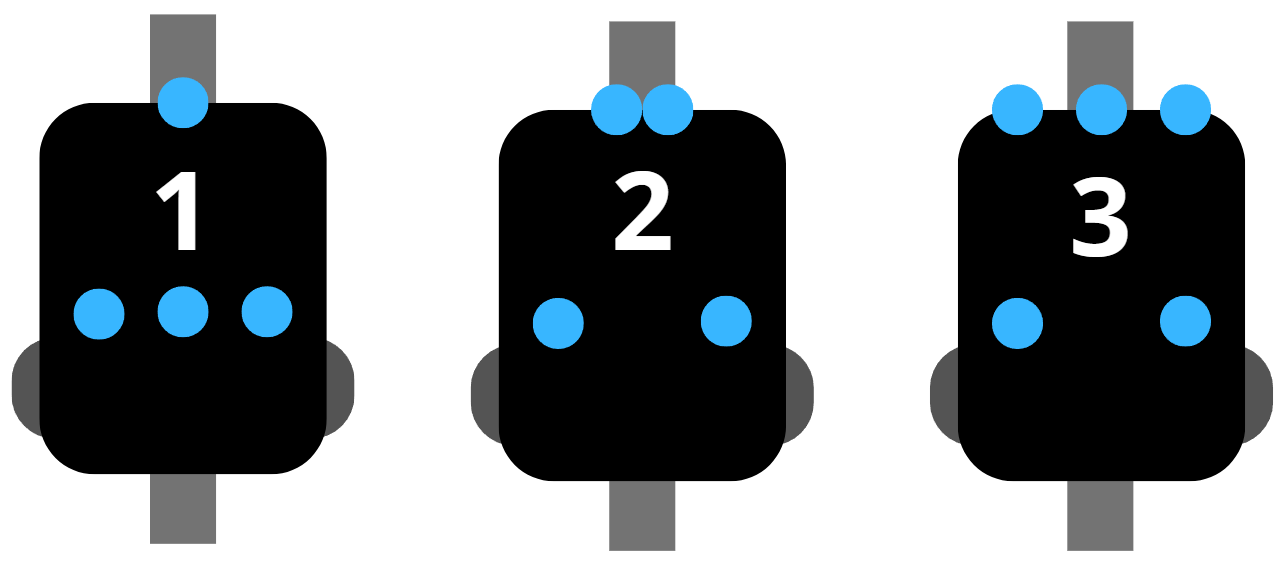
\includegraphics[width=0.9\textwidth]{images/disposition_capteurs.png}
    \caption{Différentes phases de conception et de disposition des capteurs}
\end{figure}

Les capteurs de ligne TCRT5000 sont positionnés à l’avant du robot afin de détecter la trajectoire à suivre. Leur disposition comprend un capteur central, des capteurs latéraux avant et des capteurs latéraux arrière, ce qui permet une détection précise de la ligne, y compris dans les virages et aux intersections. La figure 2.2 présente nos différentes phases de disposition de ces capteurs, ayant débuté par le 1 puis ayant opté pour la disposition 3, après de nombreux tests notamment au niveau du suivi de ligne. Les capteurs de détection d'intersection n'ont jamais bougé depuis notre réflexion initiale.


Chaque capteur est relié à un GPIO distinct du Raspberry Pi, permettant une lecture indépendante de chaque signal. Les fils de connexion sont organisés de manière à limiter les interférences, faciliter la maintenance et assurer une identification claire de chaque capteur.

Le capteur de couleur et l’écran LCD utilisent le bus de communication I2C, ce qui réduit le nombre de fils nécessaires et simplifie le câblage global du système.


\section{Bilan de puissance et estimation de l'autonomie}

Cette section présente l'estimation de l'autonomie du système robotique, divisée en deux circuits distincts : le circuit logique (alimenté par USB 5V) et le circuit de puissance (alimenté par les cellules Lithium 8.4V).

\subsection{Circuit Logique (Batterie Externe USB)}

\textbf{Données de la source :}
\begin{itemize}
    \item Capacité nominale ($C_{USB}$) : $10\,000 \text{ mAh}$
    \item Tension : $5 \text{ V}$
\end{itemize}

\textbf{Consommation des composants (sous 5V) :}
Pour les composants fonctionnant en 3.3V (capteurs, buzzer) nous considérons le courant tiré sur le rail 5V ce qui est une approximation.

\begin{enumerate}
    \item Raspberry Pi 4 : $I_{pi} = 1.25 \text{ A} = 1250 \text{ mA}$
    \item Capteurs de ligne (x5) : $I_{ligne} = 5 \times 20 \text{ mA} = 100 \text{ mA}$
    \item Capteur RGB : $I_{rgb} = 16 \text{ mA}$
    \item Écran LCD : $I_{lcd} = 50 \text{ mA}$
    \item Buzzer (activé) : $I_{buz} = 20 \text{ mA}$
\end{enumerate}

Le courant total consommé par la logique est calculé comme suit :

\begin{equation}
    I_{logique} = I_{pi} + I_{ligne} + I_{rgb} + I_{lcd} + I_{buz}
\end{equation}
\begin{equation}
    I_{logique} = 1250 + 100 + 16 + 50 + 20 = 1436 \text{ mA}
\end{equation}

\textbf{Estimation de l'autonomie ($T_{logique}$) :}
Note : Les batteries externes sont souvent notées pour la capacité de leurs cellules internes (3.7V). Pour obtenir du 5V, un convertisseur est utilisé. Nous appliquons un coefficient de rendement global réaliste $\eta \approx 0.7$ (comprenant la conversion 3.7V vers 5V et les pertes thermiques).

\begin{equation}
    T_{logique} \approx \frac{C_{USB} \times \eta}{I_{logique}} = \frac{10000 \times 0.7}{1436}
\end{equation}
\begin{equation}
    T_{logique} \approx \frac{7000}{1436} \approx \mathbf{4.87 \text{ heures}}
\end{equation}

\subsection{Circuit de Puissance (Cellules Lithium)}

\textbf{Données de la source :}
\begin{itemize}
    \item Capacité ($C_{bat}$) : $3400 \text{ mAh}$
    \item Tension : $8.4 \text{ V}$
\end{itemize}

\textbf{Consommation des composants :}
\begin{enumerate}
    \item Moteurs (x2) : $I_{mot} = 2 \times 90 \text{ mA} = 180 \text{ mA}$
    \item Contrôleur L293D : $I_{driver} = 500 \text{ mA}$
\end{enumerate}

Le courant total du circuit de puissance est :

\begin{equation}
    I_{puissance} = I_{mot} + I_{driver} = 180 + 500 = 680 \text{ mA}
\end{equation}

\textbf{Estimation de l'autonomie ($T_{puissance}$) :}
Pour des cellules Li-Ion en série, la capacité en mAh reste celle d'une seule cellule (3400 mAh), seule la tension s'additionne.

\begin{equation}
    T_{puissance} = \frac{C_{bat}}{I_{puissance}} = \frac{3400}{680}
\end{equation}
\begin{equation}
    T_{puissance} \approx \mathbf{5.0 \text{ heures}}
\end{equation}

\subsection{Conclusion}

L'autonomie globale du système est limitée par le maillon le plus faible.
\begin{itemize}
    \item Autonomie Logique (estimée avec pertes) : $\approx 4h52$
    \item Autonomie Moteurs : $\approx 5h00$
\end{itemize}

Le système devrait donc avoir une autonomie théorique d'environ \textbf{4 heures et 50 minutes} en fonctionnement continu maximal.

\section{Difficultés rencontrées et pistes d'amélioration}

Nous avons rencontré quelques difficultés, notamment :
\begin{itemize}
    \item Trouver un positionnement des capteurs optimal et en choisir le nombre adéquat
    \item Calibrer les capteurs de ligne et le capteur RGB en fonction des conditions de lumière de la salle qui ne sont jamais les mêmes.
    \item Brancher de manière fiable les câbles
\end{itemize}

Améliorations possibles :
\begin{itemize}
    \item Visser les capteurs au châssis au lieu de les scotcher
    \item Utiliser des câbles plus longs pour mieux organiser l'intérieur du robot.
\end{itemize}


\section{Flowchart}
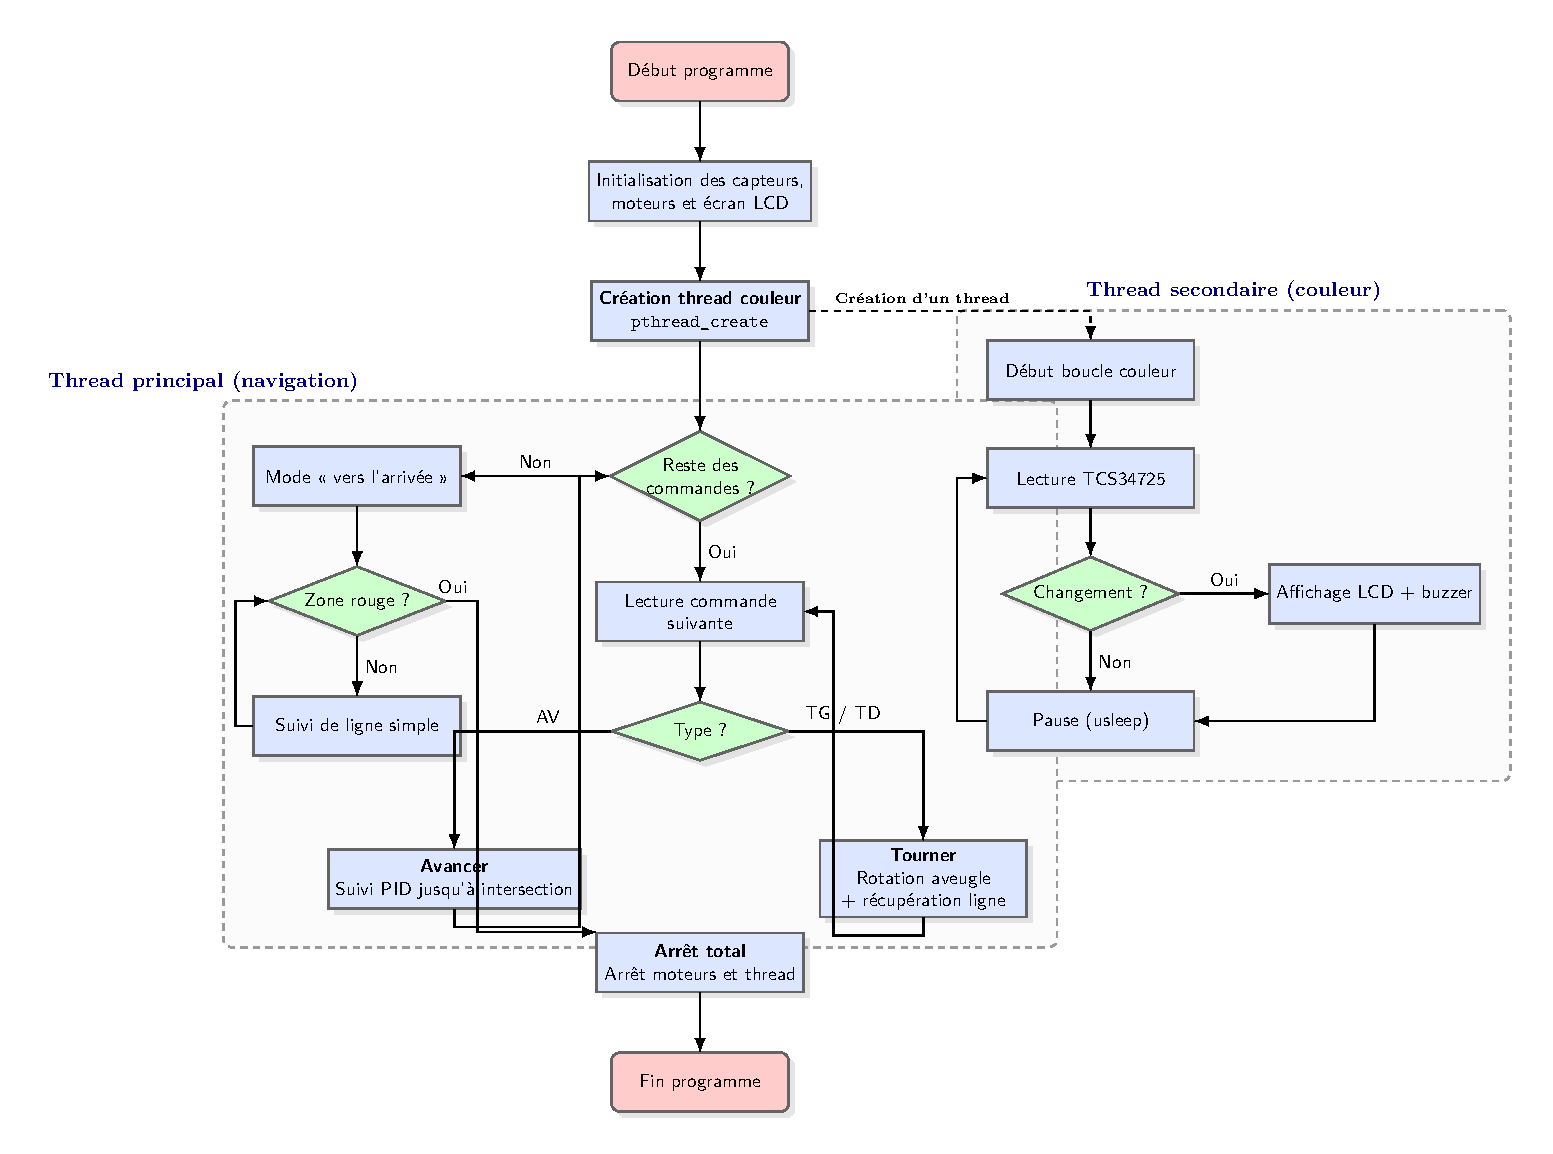
\includegraphics[height=16cm, keepaspectratio,angle=90]{images/flowchart.pdf}

% -------------------------------
% CHAPITRE 3 — Partie informatique
% -------------------------------
\chapter{Partie informatique}

\subsection{Analyse}

Cette phase d’analyse a pour objectif d’identifier les éléments fondamentaux nécessaires à la conception du programme. Le projet consiste à faire évoluer un robot dans un labyrinthe en lui fournissant une suite d’ordres cohérente, tout en respectant les contraintes imposées par la structure du labyrinthe et les règles de déplacement.

Avant de détailler les structures de données complexes et les algorithmes de recherche, il est nécessaire d’introduire les éléments de base utilisés dans les types abstraits de données. Ces éléments constituent le socle de la modélisation et interviennent directement dans la définition des opérations de déplacement du robot.

\subsubsection{Types}

Dans cette première étape de conception, seul le type \textbf{Direction} est introduit. Il s’agit d’une énumération regroupant les quatre directions cardinales : Nord, Est, Sud et Ouest.

Ce type permet de représenter l’orientation du robot dans le labyrinthe. L’orientation joue un rôle central dans la navigation, car elle conditionne les mouvements possibles à partir d’une position donnée. Par exemple, la notion de « case devant le robot » dépend directement de la direction dans laquelle celui-ci est orienté.

L’utilisation d’une énumération dédiée présente plusieurs avantages. Elle garantit que seules des directions valides peuvent être manipulées, améliore la lisibilité des algorithmes et facilite la définition des règles de déplacement, telles que les rotations à gauche ou à droite. Ce type est utilisé directement dans les types abstraits définis par la suite, notamment ceux liés au robot et à la gestion des états.

\subsubsection{TAD}
Avant de passer à l'analyse descendante, nous allons aborder les TAD introduits : Labyrinthe et Robot. Commençons par le TAD Labyrinthe :

\begin{tad}

\tadNom{Labyrinthe}

\tadParametres{}

\tadDependances{
Graphe$\langle$Sommet = NNN, Etiquette = NNN$\rangle$,
Ensemble$\langle$NNN$\rangle$,
Liste$\langle$NNN$\rangle$,
\booleen,
\naturel,
NNN
}

\begin{tadOperations}{retirerSommetCommePassage}

\tadOperation{labyrinthe}
{\tadUnParam{NNN}}
{\tadUnParam{Labyrinthe}}

\tadOperation{obtenirTaille}
{\tadUnParam{Labyrinthe}}
{\tadUnParam{NNN}}

\tadOperation{obtenirNbSommets}
{\tadUnParam{Labyrinthe}}
{\tadUnParam{\naturel}}

\tadOperation{ajouterChemin}
{\tadTroisParams{Labyrinthe}{NNN}{NNN}}
{\tadUnParam{Labyrinthe}}

\tadOperation{retirerChemin}
{\tadTroisParams{Labyrinthe}{NNN}{NNN}}
{\tadUnParam{Labyrinthe}}

\tadOperation{estUnSommetPassage}
{\tadDeuxParams{Labyrinthe}{NNN}}
{\tadUnParam{\booleen}}

\tadOperation{marquerSommetCommePassage}
{\tadDeuxParams{Labyrinthe}{NNN}}
{\tadUnParam{Labyrinthe}}

\tadOperation{retirerSommetCommePassage}
{\tadDeuxParams{Labyrinthe}{NNN}}
{\tadUnParam{Labyrinthe}}

\tadOperation{obtenirSommetsPassage}
{\tadUnParam{Labyrinthe}}
{\tadUnParam{Ensemble$\langle$NNN$\rangle$}}

\tadOperation{obtenirSommetsAdjacents}
{\tadDeuxParams{Labyrinthe}{NNN}}
{\tadUnParam{Ensemble$\langle$NNN$\rangle$}}

\tadOperation{estUnChemin}
{\tadTroisParams{Labyrinthe}{NNN}{NNN}}
{\tadUnParam{\booleen}}

\tadOperation{estUnVoyage}
{\tadDeuxParams{Labyrinthe}{Liste$\langle$NNN$\rangle$}}
{\tadUnParam{\booleen}}

\end{tadOperations}

\begin{tadAxiomes}

\tadAxiome{$obtenirTaille(labyrinthe(t)) = t$}

\tadAxiome{$obtenirNbSommets(labyrinthe(t)) = t \times t$}

\tadAxiome{$obtenirSommetsPassage(labyrinthe(t)) = ensembleVide()$}

\tadAxiome{$estUnSommetPassage(lab, s) =
estPresent(obtenirSommetsPassage(lab), s)$}

\tadAxiome{$estUnChemin(lab, s_1, s_2) =
appartient(obtenirSommetsAdjacents(lab, s_1), s_2)$}

\tadAxiome{$estUnChemin(lab, s_1, s_2) =
estUnChemin(lab, s_2, s_1)$}

\tadAxiome{$obtenirSommetsAdjacents(ajouterChemin(lab, s_1, s_2), s_1) = \\
ajouter(obtenirSommetsAdjacents(lab, s_1), s_2)$}

\tadAxiome{$obtenirSommetsAdjacents(ajouterChemin(lab, s_1, s_2), s_2) = \\
ajouter(obtenirSommetsAdjacents(lab, s_2), s_1)$}

\tadAxiome{$obtenirSommetsAdjacents(ajouterChemin(lab, s_1, s_2), s) = \\
obtenirSommetsAdjacents(lab, s)
\text{ si } s \neq s_1 \text{ et } s \neq s_2$}

\tadAxiome{$obtenirSommetsAdjacents(retirerChemin(lab, s_1, s_2), s_1) = \\
retirer(obtenirSommetsAdjacents(lab, s_1), s_2)$}

\tadAxiome{$obtenirSommetsAdjacents(retirerChemin(lab, s_1, s_2), s_2) = \\
retirer(obtenirSommetsAdjacents(lab, s_2), s_1)$}

\tadAxiome{$estUnVoyage(lab, l) =
estUnChemin(lab, obtenirElement(l, 1), obtenirElement(l, 2)) \\
et estUnVoyage(lab, supprimer(l, 1))
\text{ si } longueur(l) > 2$}

\tadAxiome{$estUnVoyage(lab,
ajouter(ajouter(liste(), e_1), e_2)) =
estUnChemin(lab, e_1, e_2)$}

\end{tadAxiomes}

\begin{tadPreconditions}{retirerSommetCommePassage}

\tadPrecondition{retirerSommetCommePassage(lab, s)}
{$estUnSommetPassage(lab, s)$}

\tadPrecondition{ajouterChemin(lab, s_1, s_2)}
{$non(estUnChemin(lab, s_1, s_2))$}

\tadPrecondition
{retirerChemin(lab, s_1, s_2)}
{$estUnChemin(lab, s_1, s_2)$}

\tadPrecondition
{estUnVoyage(lab, l)}
{$longueur(l) > 1$}
\end{tadPreconditions}

\end{tad}

Ensuite on peut présenter le TAD robot, qui fonctionne conjointement avec le TAD Labyrinthe :

\begin{algorithme}
\begin{tad}
\tadNom{Robot}
\tadParametres{}

\tadDependances{
Labyrinthe,
Direction,
\booleen,
NNN
}

\begin{tadOperations}{avancer}

\tadOperation{robot}
{\tadDeuxParams{NNN}{Direction}}
{\tadUnParam{Robot}}

\tadOperation{obtenirPosition}
{\tadUnParam{Robot}}
{\tadUnParam{NNN}}

\tadOperation{obtenirDirection}
{\tadUnParam{Robot}}
{\tadUnParam{Direction}}

\tadOperation{tournerGauche}
{\tadUnParam{Robot}}
{\tadUnParam{Robot}}

\tadOperation{tournerDroite}
{\tadUnParam{Robot}}
{\tadUnParam{Robot}}

\tadOperation{caseExistante}
{\tadDeuxParams{Robot}{Labyrinthe}}
{\tadUnParam{\booleen}}

\tadOperation{caseSuivante}
{\tadDeuxParams{Robot}{Labyrinthe}}
{\tadUnParam{NNN}}

\tadOperation{peutAvancer}
{\tadDeuxParams{Robot}{Labyrinthe}}
{\tadUnParam{\booleen}}

\tadOperation{avancer}
{\tadDeuxParams{Robot}{Labyrinthe}}
{\tadUnParam{Robot}}

\tadOperation{estSurSommetPassage}
{\tadDeuxParams{Robot}{Labyrinthe}}
{\tadUnParam{\booleen}}

\tadOperation{peutAllerGauche}
{\tadDeuxParams{Robot}{Labyrinthe}}
{\tadUnParam{\booleen}}

\tadOperation{peutAllerDroite}
{\tadDeuxParams{Robot}{Labyrinthe}}
{\tadUnParam{\booleen}}

\tadOperation{directionGauche}
{\tadUnParam{Robot}}
{\tadUnParam{Direction}}

\tadOperation{directionDroite}
{\tadUnParam{Robot}}
{\tadUnParam{Direction}}

\end{tadOperations}

\begin{tadAxiomes}

\tadAxiome{$obtenirPosition(robot(c, d)) = c$}
\tadAxiome{$obtenirDirection(robot(c, d)) = d$}

\tadAxiome{$obtenirPosition(tournerGauche(r)) = obtenirPosition(r)$}
\tadAxiome{$obtenirPosition(tournerDroite(r)) = obtenirPosition(r)$}

\tadAxiome{$obtenirDirection(tournerGauche(robot(s, Nord))) = Ouest$}
\tadAxiome{$obtenirDirection(tournerGauche(robot(s, Ouest))) = Sud$}
\tadAxiome{$obtenirDirection(tournerGauche(robot(s, Sud))) = Est$}
\tadAxiome{$obtenirDirection(tournerGauche(robot(s, Est))) = Nord$}

\tadAxiome{$obtenirDirection(tournerDroite(robot(s, Nord))) = Est$}
\tadAxiome{$obtenirDirection(tournerDroite(robot(s, Est))) = Sud$}
\tadAxiome{$obtenirDirection(tournerDroite(robot(s, Sud))) = Ouest$}
\tadAxiome{$obtenirDirection(tournerDroite(robot(s, Ouest))) = Nord$}

\tadAxiome{$estSurSommetPassage(r, lab) = \\
estPresent(obtenirSommetsPassage(lab), obtenirPosition(r))$}

\tadAxiome{$caseSuivante(robot(c, Nord), lab) = c - obtenirTaille(lab)$}
\tadAxiome{$caseSuivante(robot(c, Sud), lab) = c + obtenirTaille(lab)$}
\tadAxiome{$caseSuivante(robot(c, Est), lab) = c + 1$}
\tadAxiome{$caseSuivante(robot(c, Ouest), lab) = c - 1$}

\tadAxiome{$peutAvancer(r, lab) =
caseExistante(r, lab) et \\
estUnChemin(lab, obtenirPosition(r), caseSuivante(r, lab))$}

\tadAxiome{$obtenirPosition(avancer(r, lab)) = caseSuivante(r, lab)$}
\tadAxiome{$obtenirDirection(avancer(r, lab)) = obtenirDirection(r)$}

\tadAxiome{$peutAllerGauche(r, lab) = peutAvancer(tournerGauche(r), lab)$}
\tadAxiome{$peutAllerDroite(r, lab) = peutAvancer(tournerDroite(r), lab)$}

\tadAxiome{$directionGauche(r) = obtenirDirection(tournerGauche(r))$}
\tadAxiome{$directionDroite(r) = obtenirDirection(tournerDroite(r))$}

\tadAxiome{$caseExistante(r, lab) =
\Big(
obtenirPosition(r) \le obtenirNbSommets(lab)
\Big)\\
ou \Big(
\big(obtenirDirection(r)=Nord et obtenirPosition(r) > obtenirTaille(lab)\big)\\
ou \big(obtenirDirection(r)=Sud \et obtenirPosition(r) \le obtenirNbSommets(lab)-obtenirTaille(lab)\big)
ou \big(obtenirDirection(r)=Est and (obtenirPosition(r) \bmod obtenirTaille(lab)) \neq 0\big) \\
ou \big(obtenirDirection(r)=Ouest and (obtenirPosition(r) \bmod obtenirTaille(lab)) \neq 1\big)
\Big)$}

\end{tadAxiomes}

\begin{tadPreconditions}

\tadPrecondition
{caseSuivante(r, lab)}
{$caseExistante(r, lab)$}

\tadPrecondition
{avancer(r, lab)}
{$peutAvancer(r, lab)$}

\end{tadPreconditions}

\end{tad}
\end{algorithme}


\subsubsection{Analyse descendante}

Une fois ce type fondamental défini, l’analyse descendante permet de structurer la résolution du problème. L’orientation du robot, représentée par le type \textbf{Direction}, intervient dans la majorité des opérations de navigation et doit donc être intégrée dès la conception des algorithmes.

Le problème global peut être vu comme une succession de décisions dépendant à la fois de la position du robot et de son orientation. Cette observation conduit naturellement à une approche par exploration d’états, où chaque état correspond à une configuration précise du robot dans le labyrinthe.

Cette analyse constitue le fondement de la définition des types abstraits plus complexes et à la mise en place de l’algorithme de recherche utilisé pour déterminer la suite d’actions à exécuter.

\begin{figure}[h]
\centering
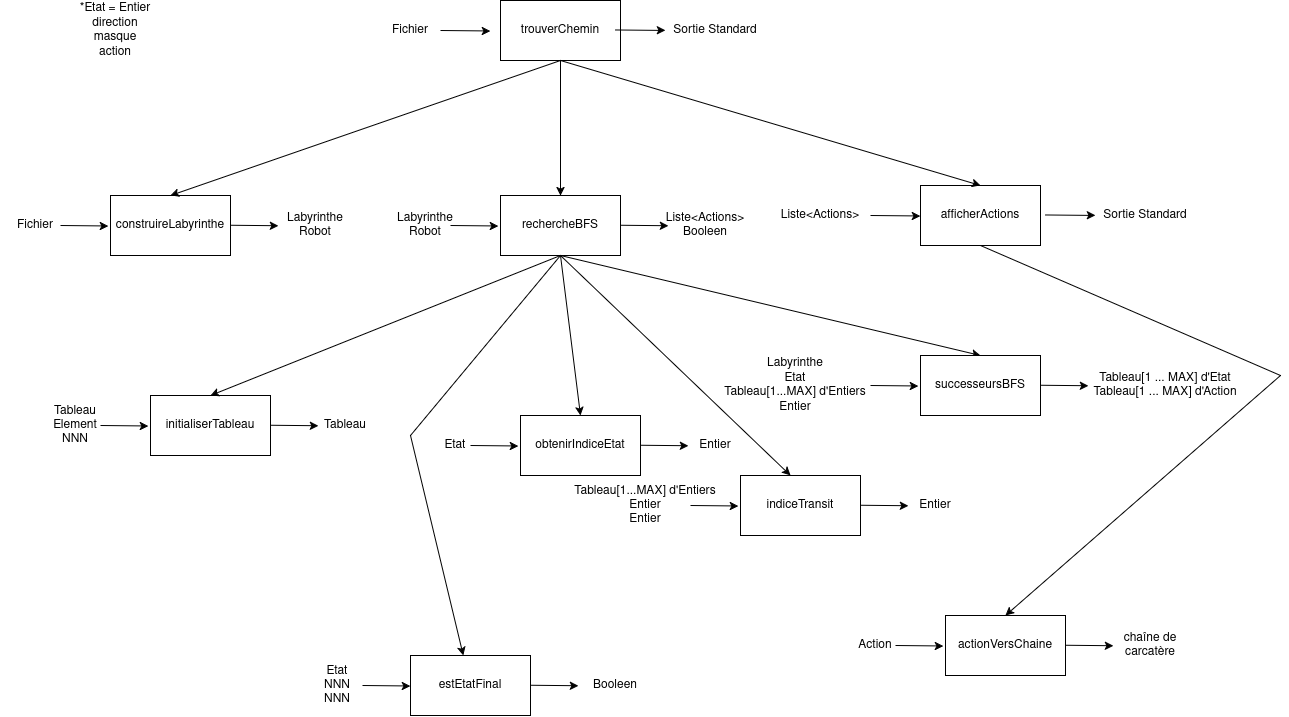
\includegraphics[width=0.8\textwidth]{AD_Final.png}
\caption{Analyse Descendante}
\label{fig:AD}
\end{figure}

\subsection{Conception Préliminaire}

Maintenant que les TAD sont définis, nous allons voir les signatures de fonctions pour l'implémentation de nos TAD. Dans un premier temps, regardons le labyrinthe, et l'implémentation pour notre programme :

\begin{algorithme}
    \begin{enregistrement}{Labyrinthe}
        \champEnregistrement{graphe}{Graphe}
        \champEnregistrement{pointsTransit}{Ensemble}
        \champEnregistrement{taille}{\entier}
    \end{enregistrement}
\end{algorithme}

Pour ces fonctions et procédure, on va reprendre les principales opérations du TAD et utiliser les fonctions et procédures suivantes :


\begin{algorithme}
    \signatureFonction{creerLabyrinthe}{taille : \entier}{Labyrinthe}{}

    \signatureFonction{obtenirTaille}{labyrinthe : Labyrinthe}{\entier}{}
    
    \signatureFonction{obtenirPointsTransit}{labyrinthe : Labyrinthe}{Ensemble}{}
    
    \signatureFonction{obtenirVoisins}{labyrinthe : Labyrinthe, source : \entier}{Ensemble}{}
    
    \signatureFonction{obtenirDegre}{labyrinthe : Labyrinthe, case : \entier}{\entier}{}

    % Modificateurs (Procédures)
    \signatureProcedure{ajouterPassage}{
        \paramEntreeSortie{labyrinthe : Labyrinthe}, \paramEntree{source, destination : \entier}
    }{}

    \signatureProcedure{supprimerPassage}{
        \paramEntreeSortie{labyrinthe : Labyrinthe}, \paramEntree{source, destination : \entier}
    }{}

    \signatureProcedure{ajouterPointTransit}{
        \paramEntreeSortie{labyrinthe : Labyrinthe}, \paramEntree{source : \entier}
    }{}

    \signatureProcedure{supprimerPointTransit}{
        \paramEntreeSortie{labyrinthe : Labyrinthe}, \paramEntree{source : \entier}
    }{}

    % Prédicats (Fonctions booléennes)
    \signatureFonction{estPassage}{labyrinthe : Labyrinthe, source, destination : \entier}{\booleen}{}
    
    \signatureFonction{estTrajet}{labyrinthe : Labyrinthe, trajet : Liste}{\booleen}{}
    
    \signatureFonction{estPointTransit}{labyrinthe : Labyrinthe, source : \entier}{\booleen}{}

    % Entrées / Sorties / Utilitaires
    \signatureProcedure{afficherLabyrinthe}{\paramEntree{labyrinthe : Labyrinthe}}{}
\end{algorithme}

\noindent On considère notre robot implémenté de la manière suivante :

\begin{algorithme}
    \type{Direction}{\{NORD, EST, SUD, OUEST\}}
\end{algorithme}
\begin{algorithme}
    % Déclaration de la structure Robot
    \begin{enregistrement}{Robot}
        \champEnregistrement{position}{\entier}
        \champEnregistrement{direction}{Direction}
    \end{enregistrement}
\end{algorithme}
Enfin on va maintenant pouvoir énoncer les différentes fonction et procédures pour le robot :

\begin{algorithme}
    \signatureFonction{creerRobot}{position : \entier, direction : Direction}{Robot}{}

    \signatureFonction{obtenirPosition}{robot : Robot}{\entier}{}

    \signatureProcedure{definirPosition}{\paramEntreeSortie{robot : Robot}, \paramEntree{position : \entier}}{}

    \signatureFonction{obtenirDirection}{robot : Robot}{Direction}{}

    \signatureProcedure{tournerGauche}{\paramEntreeSortie{robot : Robot}}{}

    \signatureProcedure{tournerDroite}{\paramEntreeSortie{robot : Robot}}{}

    \signatureFonction{caseDevantExiste}{robot : Robot, laby : Labyrinthe}{\booleen}{}

    \signatureFonction{caseSuivante}{robot : Robot, laby : Labyrinthe}{\entier}{}

    \signatureFonction{peutAvancer}{robot : Robot, laby : Labyrinthe}{\booleen}{}

    \signatureFonction{estSurPointTransit}{robot : Robot, laby : Labyrinthe}{\booleen}{}

    \signatureProcedure{avancer}{\paramEntreeSortie{robot : Robot}, \paramEntree{laby : Labyrinthe}}{}

    \signatureFonction{peutAllerGauche}{robot : Robot, laby : Labyrinthe}{\booleen}{}

    \signatureFonction{peutAllerDroite}{robot : Robot, laby : Labyrinthe}{\booleen}{}

    \signatureFonction{directionGauche}{robot : Robot}{Direction}{}

    \signatureFonction{directionDroite}{robot : Robot}{Direction}{}

    \signatureFonction{avancerJusqueVirage}{robot : Robot, labyrinthe : Labyrinthe, positions : \tableauUneDimension{1..N}{d'}{\entier}}{\entier}{}
\end{algorithme}

\vspace{0.5cm}

\noindent Pour ce qui est de l'algorithme liée à l'analyse descendante, on va introduire des structures nécéssaires, au bon déroulement de l'algorithme :

\begin{algorithme}
    % Enumération des actions possibles (robot_state_t)
    \type{ActionRobot}{\{RIEN, AVANCER, TOURNER\_GAUCHE, TOURNER\_DROITE\}}

    % Structure représentant l'état du robot à un instant T
    \begin{enregistrement}{EtatRobot}
        \champEnregistrement{case}{\entier}
        \champEnregistrement{orientation}{Direction}
        \champEnregistrement{masque}{\entier}
        \champEnregistrement{derniereAction}{ActionRobot}
    \end{enregistrement}
\end{algorithme}
\hspace{0.5cm}
\begin{algorithme}
    % Structure d'un successeur (Action + Nouvel État)
    \begin{enregistrement}{Successeur}
        \champEnregistrement{action}{ActionRobot}
        \champEnregistrement{etat}{EtatRobot}
    \end{enregistrement}
\end{algorithme}
\hspace{0.5cm}
\begin{algorithme}
    % Liste de successeurs (Tableau dynamique encapsulé)
    \begin{enregistrement}{ListeSuccesseurs}
        \champEnregistrement{elements}{\tableauUneDimension{1..N}{de}{Successeur}}
        \champEnregistrement{nombre}{\entier}
    \end{enregistrement}
\end{algorithme}
\hspace{0.5cm}
\begin{algorithme}
    \begin{enregistrement}{InfoVisite}
        \champEnregistrement{distance}{\entier}
        \champEnregistrement{indiceParent}{\entier}
        \champEnregistrement{actionParent}{ActionRobot}
    \end{enregistrement}
\end{algorithme}
\hspace{0.5cm}
\begin{algorithme}
    % Résultat de la recherche BFS
    \begin{enregistrement}{ResultatBFS}
        \champEnregistrement{actions}{Liste}
        \champEnregistrement{trouve}{\booleen}
    \end{enregistrement}
\end{algorithme}

\vspace{1cm}

\begin{algorithme}
    % Initialisation depuis un fichier
    % En C : labyrinthe_t** -> E/S en pseudocode
    \signatureFonction{construireLabyrinthe}{
        nomFichier : \chaine, 
        \paramEntreeSortie{labyrinthe : Labyrinthe}, 
        \paramEntreeSortie{robot : Robot}
    }{\booleen}{}

    % Génération des successeurs
    \signatureFonction{successeursBFS}{
        labyrinthe : Labyrinthe,
        etat : EtatRobot,
        pointsTransit : \tableauUneDimension{1..MAX}{d'}{\entier},
        nbPoints : \entier
    }{ListeSuccesseurs}{}

    % Algorithme principal de recherche
    \signatureFonction{rechercheBFS}{
        labyrinthe : Labyrinthe,
        robot : Robot
    }{ResultatBFS}{}

    % Affichage
    \signatureProcedure{afficherActions}{
        \paramEntree{actions : Liste},
        \paramEntree{fichierSortie : Fichier}
    }{}
\end{algorithme}
\vspace{0.5cm}
Pour faire un point sur les différentes structures, l'important est de retenir que l'on peut stocker l'état d'un robot à un instant T (position, direction, masque, dernière action). Ainsi on peut également avec Successeur noter le nouvel état d'un robot associé à une action. Enfin on peut stocker une liste de ces successeurs. Pour le parcours, infoVisite est une structure qui va noter la distance et l'indice parent associé à un état,  cette structure sera très utile pour le backtracking. Enfin une structure de résultat est présente par confort pour l'implémentation principalement.

\vspace{0.5cm}
\noindent Afin d’expliquer le fonctionnement de l’algorithme, que l'on va implémenter, on va réaliser un parcours en profondeur des états du Robot. Concrètement, pour faire le BFS :
\begin{itemize}
    \item On initialise une file avec l'état initial (défini par le robot)
    \item Tant que l'on à pas fait le parcours, on défile un état de la file
    \item On calcule tous les nouveaux états possible non visités à partir de cet état
    \item Une fois un état final trouvé, on remonte les états du point d'arrivée vers le point de départ pour reconstruire le schéma
\end{itemize}

\section{Conception détaillée }

\subsection{Fonctions du Labyrinthe}
\begin{algorithme}
\fonction{creerLabyrinthe}{n : \entier}{Labyrinthe}{n : NNN \\ L : Labyrinthe \\ i : \entier}
{
\affecter{\champ{L}{taille}}{n}
\affecter{\champ{L}{g}}{{graphe()}}
\affecter{\champ{L}{passages}}{{ensemble()}}

\pour{i}{1}{n*n}{}{
  \instruction{ajouterSommet(\champ{L}{g}, i)}
}
\retourner{L}
}
\end{algorithme}
\vspace{0.5cm}
\begin{algorithme}
\fonction{estTrajet}{L : Labyrinthe, trajet : Liste<NNN>}{\booleen}{u,v : NNN \\ i : \entier}
{
\sialors{{Liste.longueur(trajet)} < 2}{
  \retourner{faux}
}{}

\pour{i}{1}{{longueur(trajet)}-1}{}{
  \affecter{u}{{obtenirElement(trajet, i)}}
  \affecter{v}{{obtenirElement(trajet, i+1)}}
  \sialors{{non estChemin(L,u,v)}}{
    \retourner{faux}
  }{}
}
\retourner{vrai}
}
\end{algorithme}

\subsection{Fonctions du Robot}
\begin{algorithme}
\fonction{creerRobot}{pos : \entier, dir : Direction}{Robot}
{R : Robot}
{
  \affecter{\champ{R}{position}}{pos}
  \affecter{\champ{R}{direction}}{dir}
  \retourner{R}
}
\end{algorithme}

\vspace{0.5cm}

\begin{algorithme}
\fonction{caseDevantExiste}{R : Robot, L : Labyrinthe}{\booleen}
{n : \entier \\ p : \entier \\ lig, col : \entier}
{
  \affecter{n}{obtenirTaille(L)}
  \affecter{p}{obtenirPosition(R)}
  \affecter{lig}{((p-1) \mbox{div} n)+1}
  \affecter{col}{((p-1) \mbox{mod} n)+1}

  \sialors{\champ{R}{direction} = NORD}{
    \retourner{lig > 1}
  }{}
  \sialors{\champ{R}{direction} = SUD}{
    \retourner{lig < n}
  }{}
  \sialors{\champ{R}{direction} = EST}{
    \retourner{col < n}
  }{}
  \commentaire{OUEST}
  \retourner{col > 1}
}
\end{algorithme}
\vspace{0.5cm}
\begin{algorithme}
\fonction{caseSuivante}{R : Robot, L : Labyrinthe}{\entier}
{n : \entier \\ p : \entier}
{
  \affecter{n}{\champ{L}{taille}}
  \affecter{p}{\champ{R}{position}}

  \sialors{\champ{R}{direction} = NORD}{
    \retourner{p - n}
  }{}
  \sialors{\champ{R}{direction} = SUD}{
    \retourner{p + n}
  }{}
  \sialors{\champ{R}{direction} = EST}{
    \retourner{p + 1}
  }{}
  \commentaire{OUEST}
  \retourner{p - 1}
}
\end{algorithme}
\vspace{0.5cm}
\begin{algorithme}
\fonction{peutAvancer}{R : Robot, L : Labyrinthe}{\booleen}
{p : \entier \\ q : \entier}
{
  \sialors{{non caseDevantExiste(R,L)}}{
    \retourner{faux}
  }{}

  \affecter{p}{\champ{R}{position}}
  \affecter{q}{{caseSuivante(R,L)}}
  \retourner{estUnChemin(L, p, q)}
}
\end{algorithme}

\vspace{0.5cm}

\begin{algorithme}
\procedure{avancer}{
\paramEntreeSortie{R : Robot}
\paramEntree{L : Labyrinthe}
}{}{
  \sialors{{peutAvancer(R,L)}}{
    \affecter{\champ{R}{position}}{{caseSuivante(R,L)}}
  }{}
}
\end{algorithme}

\vspace{0.5cm}

\begin{algorithme}
\fonction{avancerJusqueVirage}{R : Robot, L : Labyrinthe}{\tableauUneDimension{1..MAX}{de NNN}, Entier}
{chemin : \tableauUneDimension{1..MAX}{de NNN} \\ i : Entier}
{
  \affecter{i}{1}
  \tantque{{peutAvancer(R,L)}}{
    \instruction{avancer(R,L)}
    \affecter{chemin[i]}{obtenirPosition(R)}

    \commentaire{Stop si on arrive à un embranchement (degré $\neq$ 2)}
    \sialors{{{obtenirDegre(L, \champ{R}{position})} $\neq$ 2}}{
      \retourner{chemin, i}
    }{}
      \affecter{i}{i+1}
  }

  \retourner{chemin, i}
}

\end{algorithme}

\subsection{Algorithme générale}
\vspace{0.5cm}
\begin{algorithme}
\fonction{InfoVisiteInvalide}{}{InfoVisite}
{iv : InfoVisite}
{
  \affecter{\champ{iv}{distance}}{-1}
  \affecter{\champ{iv}{indiceParent}}{-1}
  \affecter{\champ{iv}{actionParent}}{RIEN}
  \retourner{iv}
}
\end{algorithme}

\vspace{0.5cm}

\begin{algorithme}
\procedure{initialiserTableau}{
\paramEntreeSortie{t : \tableauUneDimension{0..MAX}{de}{T}}
\paramEntree{val : T, n : \entier}
}
{i : \entier}
{
  \pour{i}{1}{n}{}{
    \affecter{t[i]}{val}
  }
}
\end{algorithme}
\vspace{0.5cm}

\begin{algorithme}
\fonction{indexEtat}{e : EtatRobot, nbMasques : NNN}{\entier}
{o : \entier \\ idx : \entier \\ c0 : \entier}
{
  \commentaire{Encodage de l'orientation en 0..3}
  \sialors{\champ{e}{orientation} = NORD}{\affecter{o}{0}}{}
  \sialors{\champ{e}{orientation} = EST}{\affecter{o}{1}}{}
  \sialors{\champ{e}{orientation} = SUD}{\affecter{o}{2}}{}
  \sialors{\champ{e}{orientation} = OUEST}{\affecter{o}{3}}{}

  \affecter{c0}{\champ{e}{case} - 1}

  \commentaire{Indexation : ((case * 4) + orientation) * nbMasques + masque}
  \affecter{idx}{c0}
  \affecter{idx}{idx * 4 + o}
  \affecter{idx}{idx * nbMasques + \champ{e}{masque}}

  \retourner{idx}
}
\end{algorithme}


\vspace{0.5cm}

\begin{algorithme}
\fonction{estEtatFinal}{e : EtatRobot, masqueBut, nbMasques : NNN}{\booleen}
{}
{
  \sialors{\champ{e}{masque} < 0}{
    \retourner{faux}
  }{}
  \sialors{\champ{e}{masque} $\ge$ nbMasques}{
    \retourner{faux}
  }{}
  \retourner{\champ{e}{masque} = masqueBut}
}
\end{algorithme}
\vspace{0.5cm}

\begin{algorithme}
\fonction{successeursBFS}{
    lab : Labyrinthe,
    e : EtatRobot,
    points : \tableauUneDimension{1..nbPoints}{de NNN},
    nbPoints : \entier
}{ListeSuccesseurs}
{
  succ : ListeSuccesseurs \\
  r, r2 : Robot \\
  e2 : EtatRobot \\
  chemin : \tableauUneDimension{1..MAX}{de NNN} \\
  k : \entier \\
  i, j : \entier
}
{
  \commentaire{Reconstruire le robot depuis l'état}
  \affecter{r}{robot(\champ{e}{case}, \champ{e}{orientation})}

  \commentaire{1) Successeur : AVANCER (condensé jusqu'au virage)}
  \sialors{peutAvancer(r, lab)}{
    \commentaire{On avance le robot r en place ; chemin contient les cases traversées}
    \affecter{r2}{r}
    \affecter{(chemin, k)}{avancerJusqueVirage(r2, lab)}

    \commentaire{Construire le nouvel état e2}
    \affecter{\champ{e2}{case}}{obtenirPosition(r)+k}
    \affecter{\champ{e2}{orientation}}{obtenirDirection(r)}
    \affecter{\champ{e2}{masque}}{\champ{e}{masque}}
    \affecter{\champ{e2}{derniereAction}}{AVANCER}

    \commentaire{Mise à jour du masque : on marque tous les points atteints sur le chemin}
    \pour{j}{1}{k}{}{
      \pour{i}{1}{nbPoints}{}{
        \sialors{chemin[j] = points[i]}{
          \affecter{\champ{e2}{masque}}{\champ{e2}{masque} \textbf{OR} (1 \ll (i-1))}
        }{}
      }
    }

    \instruction{ListeSuccesseurs.ajouter(succ, AVANCER, e2)}
  }{}

  \commentaire{2) Successeur : TOURNER\_GAUCHE}
  \affecter{r2}{tournerGauche(r)}
  \affecter{\champ{e2}{case}}{\champ{e}{case}}
  \affecter{\champ{e2}{orientation}}{obtenirDirection(r2)}
  \affecter{\champ{e2}{masque}}{\champ{e}{masque}}
  \affecter{\champ{e2}{derniereAction}}{TOURNER\_GAUCHE}
  \instruction{ListeSuccesseurs.ajouter(succ, TOURNER\_GAUCHE, e2)}

  \commentaire{3) Successeur : TOURNER\_DROITE}
  \affecter{r2}{tournerDroite(r)}
  \affecter{\champ{e2}{case}}{\champ{e}{case}}
  \affecter{\champ{e2}{orientation}}{obtenirDirection(r2)}
  \affecter{\champ{e2}{masque}}{\champ{e}{masque}}
  \affecter{\champ{e2}{derniereAction}}{TOURNER\_DROITE}
  \instruction{ListeSuccesseurs.ajouter(succ, TOURNER\_DROITE, e2)}

  \retourner{succ}
}
\end{algorithme}
\vspace{0.5cm}

Il est important de détailler le fonctionnement du masque qui peut être légèrement contre-intuitif, le rôle du masque est de faire un suivi des cases visitées. Concrètement on va utiliser la notation binaire d'un nombre pour suivre cela. Admettons que nous ayons 3 points de passages à traverser, on va donc prendre un nombre sur 3 bits. Et passer le premier bit à 1 lorsque nous avons traversé le premier sommet, le deuxième pour le deuxième sommet, etc ... Cette solution a le mérite d'être très légère que ce soit en calcul ou en mémoire pour notre exploration.

\vspace{0.5cm}
\begin{algorithme}

\fonction{rechercheBFS}{L : Labyrinthe, R : Robot}{ResultatBFS}
{file : File<EtatRobot> \\
 visites : \tableauUneDimension{1..MAX}{de}{InfoVisite} \\
 vu : \tableauUneDimension{1..MAX}{de}{\booleen} \\
 etat0, etat, s : EtatRobot \\
 idx0, idx, idxs, taille : \entier \\
 trouve : \booleen \\
 idxFinal : \entier \\
 succ : ListeSuccesseurs \\
 pile : Pile<ActionRobot> \\
 act : ActionRobot \\
 actions : Liste<ActionRobot> \\
 res : ResultatBFS}
{
  \commentaire{Initialisations}
  \affecter{file}{File.file()}
  \affecter{actions}{Liste.liste()}
  \affecter{pile}{Pile.pile()}
  \affecter{trouve}{faux}
  \affecter{idxFinal}{-1}
  \affecter{taille}{16*obtenirTaille(L)*obtenirTaille(L)*(puissance(2, cardinalite(obtenirPointsTransit)-1)}

  \instruction{initialiserTableau(vu, faux, taille)}
  \instruction{initialiserTableau(visites, InfoVisiteInvalide(), taille)}

\vspace{0.5cm}
  \commentaire{État initial}
  \affecter{\champ{etat0}{case}}{obtenirPosition(R)}
  \affecter{\champ{etat0}{orientation}}{obtenirDirection(R)}
  \affecter{\champ{etat0}{masque}}{0}
  \affecter{\champ{etat0}{derniereAction}}{RIEN}

  \affecter{idx0}{indexEtat(etat0)}
  \instruction{File.enfiler(file, etat0)}
  \affecter{vu[idx0]}{vrai}
  \affecter{\champ{visites[idx0]}{distance}}{0}
  \affecter{\champ{visites[idx0]}{indiceParent}}{-1}
  \affecter{\champ{visites[idx0]}{actionParent}}{RIEN}

\vspace{0.5cm}
  \commentaire{BFS}
  \tantque{non File.estVide(file)}{
    \affecter{etat}{File.defiler(file)}
    \affecter{idx}{indexEtat(etat)}

    \sialors{estEtatFinal(etat, L)}{
      \affecter{trouve}{vrai}
      \affecter{idxFinal}{idx}
      \instruction{File.vider(file)}
    }{}

\vspace{0.5cm}
    \commentaire{Successeurs}
    \affecter{succ}{successeursBFS(L, etat)}

    \pour{i}{1}{\champ{succ}{nombre}}{}{
      \affecter{s}{\champ{succ}{elements}[i].etat}
      \affecter{idxs}{indexEtat(s)}

      \sialors{non vu[idxs]}{
        \affecter{vu[idxs]}{vrai}
        \affecter{\champ{visites[idxs]}{distance}}{\champ{visites[idx]}{distance} + 1}
        \affecter{\champ{visites[idxs]}{indiceParent}}{idx}
        \affecter{\champ{visites[idxs]}{actionParent}}{\champ{succ}{elements}[i].action}
        \instruction{File.enfiler(file, s)}
      }{}
    }
  }
\vspace{0.5cm}
  \commentaire{Reconstruction avec une pile}
  \sialors{trouve}{
    \affecter{idx}{idxFinal}

    \tantque{\champ{visites[idx]}{indiceParent} $\neq$ -1}{
      \affecter{act}{\champ{visites[idx]}{actionParent}}
      \instruction{Pile.empiler(pile, act)}
      \affecter{idx}{\champ{visites[idx]}{indiceParent}}
    }

    \tantque{non Pile.estVide(pile)}{
      \affecter{act}{Pile.depiler(pile)}
      \instruction{Liste.inserer(actions, act, Liste.longueur(actions)}
    }
  }{}

  \affecter{\champ{res}{actions}}{actions}
  \affecter{\champ{res}{trouve}}{trouve}
  \retourner{res}
}

\end{algorithme}



\section{Implémentation en C}
\subsection{Organisation des fichiers}


Le répertoire principal \texttt{programmes/} regroupe l’ensemble des fichiers liés au développement logiciel du projet.
Il est organisé en deux sous-répertoires principaux correspondant aux deux grandes parties du système :
la partie algorithmique et la partie électronique.

\begin{verbatim}
programmes/
├── algo/
└── elec/
\end{verbatim}

Cette organisation permet une séparation claire entre la logique de traitement et la gestion du matériel.

\paragraph{Répertoire \texttt{algo/} — Partie algorithmique}

Le répertoire \texttt{algo/} contient l’ensemble des fichiers relatifs à la logique algorithmique du projet,
indépendamment des contraintes matérielles.

\begin{verbatim}
algo/
├── bin/
├── include/
├── include_lib/
├── lib/
├── src/
├── src_lib/
├── Doxyfile
├── makefile
└── ville.txt
\end{verbatim}

\begin{itemize}
    \item \texttt{bin/} : contient les fichiers exécutables générés après compilation de la partie algorithmique.
    
    \item \texttt{src/} : regroupe les fichiers sources en langage C (\texttt{.c}) implémentant les algorithmes principaux
    du projet (logique de décision, calculs, traitements).
    
    \item \texttt{include/} : contient les fichiers d’en-tête (\texttt{.h}) associés aux sources de \texttt{src/}.
    Ces fichiers définissent les prototypes des fonctions, les structures de données et les constantes utilisées.
    
    \item \texttt{src\_lib/} : regroupe les fichiers sources des bibliothèques internes développées pour la partie algorithmique.
    Ces bibliothèques contiennent des fonctions génériques et réutilisables.
    
    \item \texttt{include\_lib/} : contient les fichiers d’en-tête associés aux bibliothèques présentes dans \texttt{src\_lib/}.
    Il permet une séparation claire entre le code applicatif et le code de bibliothèque.
    
    \item \texttt{lib/} : regroupe les bibliothèques compilées (par exemple fichiers \texttt{.a} ou \texttt{.so})
    issues des sources de \texttt{src\_lib/}.
    
    \item \texttt{Doxyfile} : fichier de configuration utilisé par l’outil \textit{Doxygen} pour générer automatiquement
    la documentation du code source.
    
    \item \texttt{makefile} : permet d’automatiser la compilation de la partie algorithmique,
    en gérant les dépendances, la génération des bibliothèques et des exécutables.
    
    \item \texttt{ville.txt} : fichier de données utilisé comme entrée par les algorithmes
    (paramètres, description de l’environnement ou scénarios de test).
\end{itemize}

\paragraph{Répertoire \texttt{elec/} — Partie électronique}

Le répertoire \texttt{elec/} regroupe les fichiers liés à la gestion du matériel électronique
et à l’interfaçage avec les composants physiques du système.

\begin{verbatim}
elec/
├── bin/
├── include/
├── src/
├── tests/
├── deploy.sh
└── makefile
\end{verbatim}

\begin{itemize}
    \item \texttt{bin/} : contient les exécutables générés après compilation de la partie électronique.
    
    \item \texttt{src/} : regroupe les fichiers sources en langage C dédiés à la gestion du matériel
    (capteurs, actionneurs, communication avec les composants électroniques).
    
    \item \texttt{include/} : contient les fichiers d’en-tête définissant les interfaces des modules électroniques,
    les constantes matérielles et les prototypes de fonctions.
    
    \item \texttt{tests/} : regroupe les programmes de test permettant de valider le bon fonctionnement
    des différents modules électroniques de manière indépendante.
    
    \item \texttt{deploy.sh} : script permettant d’automatiser le déploiement du programme
    sur la cible matérielle (copie des fichiers, installation et exécution).
    
    \item \texttt{makefile} : gère la compilation spécifique à la partie électronique,
    en tenant compte des dépendances matérielles et des bibliothèques nécessaires.
\end{itemize}
\paragraph{Fichiers à la racine du répertoire \texttt{programmes/}}

En plus des sous-répertoires \texttt{algo/} et \texttt{elec/}, le répertoire \texttt{programmes/}
contient deux fichiers assurant la coordination globale du projet.

\begin{itemize}
    \item \texttt{makefile} : ce fichier permet d’orchestrer la compilation complète du projet.
    Il appelle les \texttt{makefile} présents dans les sous-répertoires \texttt{algo/} et \texttt{elec/},
    assurant ainsi une compilation cohérente de l’ensemble des modules du système.
    Il facilite également la gestion des dépendances entre les différentes parties du projet.

    \item \texttt{run.sh} : script d’exécution permettant de lancer automatiquement le programme
    après compilation. Il peut inclure des étapes telles que la vérification de la présence des exécutables,
    le choix du mode d’exécution ou le lancement séquentiel des différentes parties du projet.
\end{itemize}
\paragraph{Bilan}

Cette organisation en deux sous-projets distincts permet une séparation claire entre la logique algorithmique
et la gestion du matériel. Elle améliore la lisibilité du code, facilite la maintenance
et favorise une approche modulaire et évolutive du développement.

\subsection{Tests unitaires}
\subsubsection{Tests unitaires}

Les fonctions essentielles du projet ont été validées à l’aide de tests unitaires
implémentés en langage C, en s’appuyant sur la bibliothèque \texttt{CUnit}.
Ces tests ont permis de vérifier le bon fonctionnement des modules de manière isolée,
avant leur intégration dans le système global.

Deux ensembles de tests ont été réalisés :
\begin{itemize}
    \item des tests unitaires du module \texttt{labyrinthe},
    \item des tests unitaires du module \texttt{robot}.
\end{itemize}

Chaque ensemble de tests est organisé sous forme d’une suite de tests CUnit,
avec une initialisation et un nettoyage dédiés.

---

\paragraph{Outil de test utilisé}

La bibliothèque \texttt{CUnit} a été utilisée pour la mise en place des tests unitaires.
Elle permet :
\begin{itemize}
    \item la création de suites de tests,
    \item l’exécution automatique des tests,
    \item la vérification des résultats à l’aide d’assertions,
    \item l’affichage détaillé des erreurs en cas d’échec.
\end{itemize}

Les tests sont exécutés en mode verbeux afin de faciliter l’analyse des résultats.



\paragraph{Tests unitaires du module \texttt{labyrinthe}}

Les tests du module \texttt{labyrinthe} visent à vérifier la cohérence de la structure
de données représentant le labyrinthe ainsi que les opérations associées.

\begin{itemize}
    \item \textbf{Création du labyrinthe} :  
    le test vérifie que la fonction \texttt{creerLabyrinthe} alloue correctement la structure,
    initialise la taille du labyrinthe et que les ensembles internes (points de transit)
    sont vides après la création.

    \item \textbf{Ajout et vérification des passages} :  
    le test s’assure que l’ajout d’un passage entre deux cases crée bien un lien non orienté,
    vérifiable dans les deux sens à l’aide de la fonction \texttt{estPassage}.

    \item \textbf{Suppression des passages} :  
    ce test valide que la suppression d’un passage retire correctement la connexion
    entre deux cases, dans les deux directions.

    \item \textbf{Gestion des points de transit} :  
    le test vérifie l’ajout et la suppression de points de transit, ainsi que la mise à jour
    correcte de leur cardinalité et de leur présence dans l’ensemble associé.

    \item \textbf{Obtention des voisins} :  
    ce test contrôle que la fonction \texttt{obtenirVoisins} retourne exactement
    les cases adjacentes accessibles à partir d’une case donnée.

    \item \textbf{Validation d’un trajet} :  
    la fonction \texttt{estTrajet} est testée sur :
    \begin{itemize}
        \item un trajet valide (suite de cases connectées),
        \item un trajet invalide (passage inexistant),
        \item un trajet vide.
    \end{itemize}
    Le test vérifie que la continuité du chemin est correctement détectée.
\end{itemize}



\paragraph{Tests unitaires du module \texttt{robot}}

Les tests du module \texttt{robot} permettent de vérifier le comportement du robot
dans le labyrinthe, en termes de position, d’orientation et de déplacement.

\begin{itemize}
    \item \textbf{Création du robot et accesseurs} :  
    ce test vérifie l’initialisation correcte du robot, ainsi que le bon fonctionnement
    des fonctions permettant d’accéder et de modifier sa position et sa direction.

    \item \textbf{Rotations et directions relatives} :  
    les fonctions de rotation à droite et à gauche sont testées afin de vérifier
    la cohérence des orientations successives.
    Les fonctions \texttt{directionGauche} et \texttt{directionDroite} sont également validées.

    \item \textbf{Gestion des limites du labyrinthe} :  
    ce test vérifie que le robot ne peut pas accéder à une case inexistante
    lorsqu’il se trouve au bord du labyrinthe.

    \item \textbf{Déplacement et gestion des passages} :  
    le test s’assure que le robot ne peut pas avancer en l’absence de passage,
    et qu’il se déplace correctement lorsque le passage existe.

    \item \textbf{Détection des points de transit} :  
    ce test valide la détection correcte des points de transit lorsque le robot
    se trouve sur une case marquée comme telle.

    \item \textbf{Anticipation des mouvements latéraux} :  
    les fonctions permettant de vérifier la possibilité de déplacement
    à gauche ou à droite sont testées sans modifier l’état du robot.

    \item \textbf{Avancée automatique jusqu’à un virage} :  
    ce test vérifie que la fonction \texttt{avancerJusqueVirage} permet au robot
    d’avancer automatiquement le long d’un couloir jusqu’à atteindre un point
    d’arrêt ou de changement de direction, tout en mémorisant le chemin parcouru.
\end{itemize}



\paragraph{Validation et résultats}

L’ensemble des tests unitaires a été exécuté avec succès.
Les assertions utilisées permettent de détecter immédiatement toute incohérence
dans le comportement des fonctions testées.

Ces tests ont permis de valider le bon fonctionnement des modules critiques du projet
avant leur intégration dans le programme global.

\subsubsection*{Annexe -- Pseudo-code des tests unitaires (CUnit)}

\paragraph{Fichier 1 : Tests du module \texttt{labyrinthe}}

\begin{verbatim}
INCLURE stdio.h
INCLURE CUnit/Basic.h
INCLURE "labyrinthe.h"
INCLURE "copieLiberationComparaisonTypesSimples.h"

FONCTION init_suite_success() : retourne 0
FONCTION clean_suite_success() : retourne 0

TEST test_creer_labyrinthe():
    laby <- creerLabyrinthe(4)
    ASSERT_PTR_NOT_NULL_FATAL(laby)
    ASSERT_EQUAL(obtenirTaille(laby), 4)
    ASSERT_TRUE(THE_estVide(*(obtenirPointsTransit(laby))))
    libererLabyrinthe(laby)

TEST test_ajouter_et_verifier_passage():
    laby <- creerLabyrinthe(2)
    ajouterPassage(laby, 1, 2)
    ASSERT_TRUE(estPassage(laby, 1, 2))
    ASSERT_TRUE(estPassage(laby, 2, 1))
    libererLabyrinthe(laby)

TEST test_supprimer_passage():
    laby <- creerLabyrinthe(2)
    ajouterPassage(laby, 1, 2)
    supprimerPassage(laby, 1, 2)
    ASSERT_FALSE(estPassage(laby, 1, 2))
    ASSERT_FALSE(estPassage(laby, 2, 1))
    libererLabyrinthe(laby)

TEST test_transit_points():
    laby <- creerLabyrinthe(3)
    ajouterPointTransit(laby, 3)
    ajouterPointTransit(laby, 5)
    ASSERT_TRUE(estPointTransit(laby, 3))
    ASSERT_TRUE(estPointTransit(laby, 5))
    ASSERT_EQUAL(THE_cardinalite(*(obtenirPointsTransit(laby))), 2)
    supprimerPointTransit(laby, 3)
    ASSERT_FALSE(estPointTransit(laby, 3))
    ASSERT_EQUAL(THE_cardinalite(*(obtenirPointsTransit(laby))), 1)
    libererLabyrinthe(laby)

TEST test_obtenir_voisins():
    laby <- creerLabyrinthe(3)
    ajouterPassage(laby, 1, 2)
    ajouterPassage(laby, 1, 4)
    voisins <- obtenirVoisins(laby, 1)
    voisinA <- 2
    voisinB <- 4
    nonVoisin <- 5
    ASSERT_EQUAL(THE_cardinalite(voisins), 2)
    ASSERT_TRUE(THE_estPresent(voisins, &voisinA))
    ASSERT_TRUE(THE_estPresent(voisins, &voisinB))
    ASSERT_FALSE(THE_estPresent(voisins, &nonVoisin))
    THE_vider(&voisins)
    libererLabyrinthe(laby)

TEST test_est_trajet():
    laby <- creerLabyrinthe(3)
    ajouterPassage(laby, 1, 2)
    ajouterPassage(laby, 2, 3)

    valide <- LCL_liste(CLCTS_copierInt, CLCTS_libererInt)
    n1 <- 1 ; n2 <- 2 ; n3 <- 3
    LCL_inserer(&valide, &n1, 0)
    LCL_inserer(&valide, &n2, 1)
    LCL_inserer(&valide, &n3, 2)
    ASSERT_TRUE(estTrajet(laby, &valide))

    invalide <- LCL_liste(CLCTS_copierInt, CLCTS_libererInt)
    n4 <- 4
    LCL_inserer(&invalide, &n1, 0)
    LCL_inserer(&invalide, &n4, 1)
    ASSERT_FALSE(estTrajet(laby, &invalide))

    vide <- LCL_liste(CLCTS_copierInt, CLCTS_libererInt)
    ASSERT_FALSE(estTrajet(laby, &vide))

    LCL_vider(&valide)
    LCL_vider(&invalide)
    LCL_vider(&vide)
    libererLabyrinthe(laby)

PROGRAMME PRINCIPAL main(argc, argv):
    initialiser registre de tests CUnit
    ajouter suite "Tests boite noire : labyrinthe"
    ajouter tests:
        - test_creer_labyrinthe
        - test_ajouter_et_verifier_passage
        - test_supprimer_passage
        - test_transit_points
        - test_obtenir_voisins
        - test_est_trajet
    lancer les tests en mode verbeux
    afficher les échecs
    nettoyer registre CUnit
    retourner code d’erreur
\end{verbatim}



\paragraph{Fichier 2 : Tests du module \texttt{robot}}

\begin{verbatim}
INCLURE stdio.h
INCLURE stdlib.h
INCLURE CUnit/Basic.h
INCLURE "robot.h"
INCLURE "labyrinthe.h"

FONCTION init_suite_robot() : retourne 0
FONCTION clean_suite_robot() : retourne 0

TEST test_creation_et_getters():
    robot <- creerRobot(5, NORD)
    ASSERT_PTR_NOT_NULL_FATAL(robot)
    ASSERT_EQUAL(obtenirPosition(robot), 5)
    ASSERT_EQUAL(obtenirDirection(robot), NORD)
    definirPosition(robot, 10)
    ASSERT_EQUAL(obtenirPosition(robot), 10)
    libererRobot(robot)

TEST test_rotations():
    robot <- creerRobot(1, NORD)

    tournerDroite(robot)  -> ASSERT direction == EST
    tournerDroite(robot)  -> ASSERT direction == SUD
    tournerDroite(robot)  -> ASSERT direction == OUEST
    tournerDroite(robot)  -> ASSERT direction == NORD

    tournerGauche(robot)  -> ASSERT direction == OUEST

    ASSERT_EQUAL(directionGauche(robot), SUD)
    ASSERT_EQUAL(directionDroite(robot), NORD)

    libererRobot(robot)

TEST test_limites_grille():
    laby <- creerLabyrinthe(3)
    robot <- creerRobot(2, NORD)
    ASSERT_FALSE(caseDevantExiste(robot, laby))

    definirPosition(robot, 4)
    tournerGauche(robot)  // direction OUEST
    ASSERT_FALSE(caseDevantExiste(robot, laby))

    definirPosition(robot, 5)
    ASSERT_TRUE(caseDevantExiste(robot, laby))
    ASSERT_EQUAL(caseSuivante(robot, laby), 4)

    libererLabyrinthe(laby)
    libererRobot(robot)

TEST test_mouvement_et_passages():
    laby <- creerLabyrinthe(3)
    robot <- creerRobot(1, EST)

    ASSERT_FALSE(peutAvancer(robot, laby))
    ASSERT_FALSE(avancer(robot, laby))
    ASSERT_EQUAL(obtenirPosition(robot), 1)

    ajouterPassage(laby, 1, 2)
    ASSERT_TRUE(peutAvancer(robot, laby))
    ASSERT_TRUE(avancer(robot, laby))
    ASSERT_EQUAL(obtenirPosition(robot), 2)

    libererLabyrinthe(laby)
    libererRobot(robot)

TEST test_points_transit_robot():
    laby <- creerLabyrinthe(3)
    robot <- creerRobot(5, NORD)

    ASSERT_FALSE(estSurPointTransit(robot, laby))
    ajouterPointTransit(laby, 5)
    ASSERT_TRUE(estSurPointTransit(robot, laby))

    libererLabyrinthe(laby)
    libererRobot(robot)

TEST test_regarder_cote():
    laby <- creerLabyrinthe(3)
    robot <- creerRobot(5, NORD)

    ajouterPassage(laby, 5, 4)
    ASSERT_TRUE(peutAllerGauche(robot, laby))
    ASSERT_FALSE(peutAllerDroite(robot, laby))

    ASSERT_EQUAL(obtenirPosition(robot), 5)
    ASSERT_EQUAL(obtenirDirection(robot), NORD)

    libererLabyrinthe(laby)
    libererRobot(robot)

TEST test_avancer_jusque_virage():
    laby <- creerLabyrinthe(5)
    robot <- creerRobot(1, EST)
    chemin <- NULL

    ajouterPassage(laby, 1, 2)
    ajouterPassage(laby, 2, 3)
    ajouterPassage(laby, 3, 4)

    nb_pas <- avancerJusqueVirage(robot, laby, &chemin)

    ASSERT_EQUAL(nb_pas, 3)
    ASSERT_PTR_NOT_NULL(chemin)
    SI chemin != NULL:
        ASSERT_EQUAL(chemin[0], 2)
        ASSERT_EQUAL(chemin[1], 3)
        ASSERT_EQUAL(chemin[2], 4)
        free(chemin)

    ASSERT_EQUAL(obtenirPosition(robot), 4)

    libererLabyrinthe(laby)
    libererRobot(robot)

PROGRAMME PRINCIPAL main():
    initialiser registre de tests CUnit
    ajouter suite "Tests Robot"
    ajouter tests:
        - test_creation_et_getters
        - test_rotations
        - test_limites_grille
        - test_mouvement_et_passages
        - test_points_transit_robot
        - test_regarder_cote
        - test_avancer_jusque_virage
    lancer les tests en mode verbeux
    afficher les échecs
    nettoyer registre CUnit
    retourner code d’erreur
\end{verbatim}

\subsection{Documentation}

Afin de documenter le code source du projet \textit{smartrobot}, une documentation
automatique a été générée à l’aide de l’outil \texttt{Doxygen}.
Cette approche permet de produire une documentation claire et cohérente,
directement à partir des fichiers d’en-tête du projet.


\paragraph{Objectif de la documentation}

La documentation générée vise à décrire l’API du projet, en particulier
les modules \texttt{labyrinthe} et \texttt{robot}.
Elle facilite la compréhension des structures de données et des fonctions
mises à disposition, aussi bien pour l’utilisation que pour la maintenance
du code.



\paragraph{Configuration de Doxygen}

La génération de la documentation est pilotée par un fichier de configuration
\texttt{Doxyfile}, dont le contenu a été volontairement simplifié afin
d’éviter toute interaction lors de l’exécution.

Le projet est identifié par les paramètres suivants :
\begin{itemize}
    \item \texttt{PROJECT\_NAME} : définit le nom du projet (\textit{smartrobot}),
    \item \texttt{PROJECT\_BRIEF} : fournit une description synthétique de l’API
    (\textit{labyrinthe et robot}).
\end{itemize}

La documentation est optimisée pour le langage C, grâce à l’option
\texttt{OPTIMIZE\_OUTPUT\_FOR\_C}, et l’ensemble des entités est extrait,
y compris celles ne disposant pas de commentaires explicites
(\texttt{EXTRACT\_ALL}).



\paragraph{Périmètre analysé}

L’analyse du code est volontairement limitée aux fichiers d’en-tête
du projet :
\begin{itemize}
    \item le répertoire \texttt{include/} est spécifié comme source d’entrée,
    \item seuls les fichiers \texttt{.h} sont pris en compte,
    \item l’analyse est récursive afin d’inclure les éventuels sous-répertoires.
\end{itemize}

Ce choix permet de documenter l’interface publique du projet,
sans exposer les détails d’implémentation internes.



\paragraph{Formats de sortie}

La documentation est générée sous deux formats complémentaires :
\begin{itemize}
    \item un format \textbf{HTML}, permettant une consultation interactive
    via un navigateur web ;
    \item un format \textbf{LaTeX}, pouvant être compilé afin d’obtenir
    un document PDF.
\end{itemize}

Les fichiers générés sont placés dans le répertoire \texttt{doc/}.

\paragraph{Génération de la documentation}

La génération de la documentation est réalisée à l’aide de la commande suivante,
exécutée depuis le répertoire contenant le fichier \texttt{Doxyfile} :

\begin{verbatim}
doxygen Doxyfile
\end{verbatim}

L’exécution est silencieuse (\texttt{QUIET = YES}) et les avertissements
liés à l’absence de commentaires ne sont pas bloquants,
ce qui garantit une génération fluide de la documentation.



\paragraph{Bilan}

L’utilisation de Doxygen permet de maintenir une documentation automatiquement
synchronisée avec le code source.
Cette démarche améliore la lisibilité du projet, facilite sa prise en main
et contribue à une meilleure qualité globale du développement.


% -------------------------------
% CHAPITRE 4 — Démonstration
% -------------------------------
\chapter{Démonstration}

\section{Procédure de lancement}
\begin{enumerate}
    \item Se connecter en SSH sur la Raspberry Pi ;
    \item Cloner le dépôt Git ;
    \item Build le projet (via \texttt{make}) ;
    \item Positionner le robot sur la pastille rouge dans le bon sens ;
    \item Exécuter le script \texttt{run.sh} qui exécutera les deux programmes (cf. explications précédentes).
\end{enumerate}

\section{Mesure du temps}

\begin{verbatim}
algo git:(Algo-elec) time ./bin/laby ville.txt
AV
TG
AV
[...]
TD
AV
AV
.
./bin/laby ville.txt  0,06s user 0,00s system 98% cpu 0,060 total
\end{verbatim}
L'exécution de l'algorithme est très rapide : 60 millisecondes pour la ville du sujet.

Pour la mesure du temps du robot, nous n'avons pas réussi à terminer le parcours le jour de la soutenance. Par conséquent, nous n'avons pas de métrique à ce sujet. Néanmoins, nous avons réussi à parcourir les 15 premières cases en 30 secondes.

\section{Comportement observé}

\subsection{Première tentative}
Lors de la première, le robot a détecté la ligne entre deux plaques comme une intersection, il s'est alors mis à tourner au milieu d'une ligne droite.

\subsection{Deuxième tentative}
Lors de la deuxième tentative, le robot a parcouru sans faute les 15 premières tuiles. Il a sonné correctement au passage des pastilles, il a bien affiché toutes les instructions sur son écran. Néanmoins, à la sortie d'un virage qui était suivi d'une pastille, les capteurs n'ont pas lu la ligne noire qui était cachée par la pastille.

\subsection{Troisième tentative}
Lors de la troisième tentative, le robot s'est planté dès le premier virage pour la même raison, les capteurs avant ont besoin de passer sur la ligne noire pour arrêter la rotation mais la pastille verte cachait la ligne...

% blabla

% -------------------------------
% CHAPITRE 5 — Réalisation et gestion de projet
% -------------------------------
\include{parties/realisation_projet}

% -------------------------------
% CONCLUSION
% -------------------------------
\chapter*{Conclusion}
\addcontentsline{toc}{chapter}{Conclusion}

Ce projet intégratif nous a permis de mettre en \oe uvre de manière concrète les compétences acquises en électronique pour les systèmes embarqués et en algorithmique avancée et programmation C. L'objectif était ambitieux : concevoir un système autonome capable d'analyser une ville virtuelle, de calculer le chemin optimal et de s'y déplacer physiquement avec précision.

Sur le plan technique, nous avons réussi à concevoir une architecture matérielle fonctionnelle, validée par un bilan de puissance cohérent assurant près de 5 heures d'autonomie théorique. La séparation des circuits de puissance et de logique a garanti la stabilité du Raspberry Pi. 

Côté logiciel, l'implémentation du cycle en V nous a permis de structurer notre code efficacement. Une attention particulière a été portée à l'optimisation des tâches : l'utilisation du multithreading pour la gestion des périphériques (buzzer, écran LCD et capteur RGB) a permis de fluidifier la boucle de navigation principale, tandis que l'algorithme de recherche en largeur (BFS) s'est révélé extrêmement performant, calculant le trajet optimal en seulement 60 millisecondes.

La démonstration finale a mis en lumière à la fois la fiabilité de notre logique et les défis du monde physique. Bien que le robot ait parfaitement négocié les 15 premières cases, il a rencontré une difficulté technique liée à la détection des lignes sous les pastilles de couleur. Cet incident montre les limites du code face aux aléas de l'environnement réel.

Au-delà de l'aspect technique, ce projet a été une expérience formatrice en gestion de projet. La coordination entre les pôles électronique et informatique, ainsi que l'utilisation d'outils collaboratifs comme Git, ont été enrichissantes.

Le tableau ci-dessous détaille la répartition des tâches et les contributions de chaque membre de l'équipe ayant permis la réalisation de ce robot. Il est important de préciser que le nombre de commits de chacun n'est pas vraiment représentatif du travail fourni.

\vspace{0.5cm}

\begin{table}[H]
    \centering
    \renewcommand{\arraystretch}{1.4} % Aère les lignes (plus joli)
    \setlength{\tabcolsep}{12pt}      % Espace horizontal dans les cellules
    
    \begin{tabular}{@{} l p{8.5cm} @{}} 
    \toprule
    \textbf{Membres} & \textbf{Rôles \& Contributions} \\ 
    \midrule
    
    Assi Hadi & \multirow{2}{=}{Conception électronique, câblage, soudure, perçage du châssis, tests des composants et développement programmes composants} \\ 
    Doubet Edouard & \\ 
    \addlinespace[0.2cm] % Petit espace de séparation
    
    (El Marzouki Adam) & Gestion de projet, organisation, planning \\ 
    \addlinespace[0.2cm]
    
    Eraud-Robert Bréhan & \multirow{2}{=}{Développement informatique (Algo), structures de données (TAD), analyse descendante et Direction Artistique} \\ 
    Antunes Célia & \\ 
    \addlinespace[0.2cm]
    
    Leprevost Romain & Développement informatique (robot), test des composants et ajustements \\ 
    
    \bottomrule
    \end{tabular}
    \caption{Répartition des tâches au sein de l'équipe}
    \label{tab:repartition}
\end{table}

\section{Utilisation de l'IA / de LLM}
Dans une démarche de transparence sur l'utilisation de ces outils, nous avons documenté dans un tableau individuel dans quel cadre ces derniers ont été utilisés.

\vspace{0.5cm}

\begin{table}[H]
    \centering
    \renewcommand{\arraystretch}{1.4} % Aère les lignes (plus joli)
    \setlength{\tabcolsep}{12pt}      % Espace horizontal dans les cellules
    
    \begin{tabular}{@{} l p{12cm} @{}} 
    \toprule
    \textbf{Membres} & \textbf{Rôles \& Contributions} \\ 
    \midrule
    
    Assi Hadi & Questions concernant le branchement du bus I²C, en particulier les adresses les plus courantes de l’écran LCD et du capteur RGB, le fonctionnement du capteur RGB, ainsi que la définition de plages de valeurs RGB adaptées pour différencier les pastilles du plateau.  \\ 
    Doubet Edouard & Questions concernant les branchements sur l'I2C et les adresses les plus courantes pour l'écran LCD et le capteur RGB, questions sur le fonctionnement du capteur RGB et idées sur des valeurs RGB pour différencier les pastilles du plateau  \\ 
    (El Marzouki Adam) & N/A \\ 
    Eraud-Robert Bréhan & Base du script bash, support à la génération des tests et de la documentation. Correction de bugs de conception sur le BFS, uniformisation des noms de variables, génération de labyrinthes de test.  \\ 
    Antunes Célia & Renseignement pour les différents algorithmes qui existent pour le plus court chemin et le plus adapté. Correction de bugs et support à la génération des tests. Aide lors d'erreur de compilation inhabituelle \\ 
    Leprevost Romain & Idées de disposition capteurs / correction de problèmes liés au robot, flowchart rapport, makefile. Tentative sur le code du robot mais très insatisfaisant, besoin de connaître le robot et ses spécificités \\ 
    
    \bottomrule
    \end{tabular}
    \caption{Documentation de l'utilisation de l'IA par membre}
    \label{tab:ia}
\end{table}

\end{document}
